% Requires in the preamble:
% \usepackage{amsmath,amssymb}
% \usepackage{tikz,pgfplots}
% \pgfplotsset{compat=1.18}

\chapter{The Derivative}
\label{chap:derivative}

The last chapter ended with one limit:

\[
\lim_{h\to0}\frac{f(a+h)-f(a)}{h}.
\]

The numerator measures change in output.  The denominator measures change in input.  The quotient is an average rate of change.  The limit, if it exists, is the instantaneous rate of change.

That limit will now become a new object: the \emph{derivative}.  It is the mathematical version of what a speedometer does.  It is also the slope of a curve when we zoom in until the curve looks straight.

\section{Average rate of change}
\label{sec:average-rate-of-change}

A limit of average rates cannot be understood until the average rate itself is clear.  So we begin with the ordinary slope between two points.

If \(f\) is a function and the input changes from \(a\) to \(b\), then the output changes from \(f(a)\) to \(f(b)\).  The average rate of change compares these two changes:

\[
\frac{\text{change in output}}{\text{change in input}}
=
\frac{f(b)-f(a)}{b-a}.
\]

This is the slope of the line through the two graph points

\[
(a,f(a))
\qquad\text{and}\qquad
(b,f(b)).
\]

That line is called a secant line.

\subsection{Secant slope}
\label{subsec:secant-slope}

On a straight line, one slope tells the whole story.  On a curved graph, the slope between two points depends on which two points we choose.

Let

\[
f(x)=x^2.
\]

Between \(x=1\) and \(x=3\), the function changes from

\[
f(1)=1
\]

to

\[
f(3)=9.
\]

The average rate of change is

\[
\frac{f(3)-f(1)}{3-1}
=
\frac{9-1}{2}
=
4.
\]

So over this interval the graph rises, on average, \(4\) units of output for each \(1\) unit of input.

\begin{figure}[h]
\centering
\begin{tikzpicture}
\begin{axis}[
    width=0.76\textwidth,
    height=0.48\textwidth,
    xmin=0, xmax=3.7,
    ymin=0, ymax=11,
    axis lines=left,
    xlabel={\(x\)},
    ylabel={\(y\)},
    xtick={1,3},
    ytick={1,9},
    grid=both,
    grid style={line width=.1pt, draw=gray!25},
]
\addplot[thick, domain=0:3.4, samples=100] {x^2};
\addplot[very thick, domain=0.45:3.35, samples=2] {4*x-3};
\addplot[only marks, mark=*] coordinates {(1,1) (3,9)};
\draw[dashed] (axis cs:1,0) -- (axis cs:1,1);
\draw[dashed] (axis cs:3,0) -- (axis cs:3,9);
\draw[dashed] (axis cs:1,1) -- (axis cs:3,1);
\draw[dashed] (axis cs:3,1) -- (axis cs:3,9);
\node[anchor=east] at (axis cs:1,1.2) {\((1,1)\)};
\node[anchor=west] at (axis cs:3,9) {\((3,9)\)};
\node[anchor=south] at (axis cs:2,1.05) {\(\Delta x=2\)};
\node[anchor=west] at (axis cs:3.05,5) {\(\Delta y=8\)};
\node[anchor=west] at (axis cs:1.55,7.0) {secant slope \(=\dfrac{8}{2}=4\)};
\end{axis}
\end{tikzpicture}
\caption{The average rate of change is the slope of the secant line through two graph points.}
\label{fig:secant-slope-parabola}
\end{figure}

The symbols \(\Delta x\) and \(\Delta y\) are useful here.  The Greek letter \(\Delta\) means ``change in.''

For the example above,

\[
\Delta x=3-1=2,
\]

and

\[
\Delta y=f(3)-f(1)=9-1=8.
\]

So

\[
\text{secant slope}
=
\frac{\Delta y}{\Delta x}
=
\frac{8}{2}
=
4.
\]

\begin{quote}
\textbf{Average rate of change.}
For a function \(f\), the average rate of change from \(x=a\) to \(x=b\), where \(a\neq b\), is

\[
\boxed{
\frac{f(b)-f(a)}{b-a}.
}
\]

Geometrically, this is the slope of the secant line through \((a,f(a))\) and \((b,f(b))\).
\end{quote}

The order matters only through the signs.  If we compute from \(b\) back to \(a\), then both the numerator and denominator change sign:

\[
\frac{f(a)-f(b)}{a-b}
=
\frac{-(f(b)-f(a))}{-(b-a)}
=
\frac{f(b)-f(a)}{b-a}.
\]

So the secant slope is the same line slope either way.

\paragraph{Example.}
Find the average rate of change of

\[
f(x)=x^2
\]

from \(x=2\) to \(x=5\).

We compute

\[
\frac{f(5)-f(2)}{5-2}
=
\frac{25-4}{3}
=
7.
\]

So on the interval \([2,5]\), the function \(x^2\) increases by an average of \(7\) output units per input unit.

Notice that this does not mean the graph has slope \(7\) everywhere between \(2\) and \(5\).  Near \(x=2\), the graph is less steep.  Near \(x=5\), it is steeper.  The number \(7\) describes the whole interval at once.

\subsection{Average velocity}
\label{subsec:average-velocity}

The same quotient appears in motion.

Let \(s(t)\) be the position of an object at time \(t\).  If \(s\) is measured in meters and \(t\) is measured in seconds, then

\[
\frac{s(b)-s(a)}{b-a}
\]

has units

\[
\frac{\text{meters}}{\text{seconds}}.
\]

That is a velocity.

\begin{quote}
\textbf{Average velocity.}
If \(s(t)\) is position, then the average velocity from \(t=a\) to \(t=b\) is

\[
\boxed{
\frac{s(b)-s(a)}{b-a}.
}
\]
\end{quote}

\paragraph{Example.}
Suppose a particle moves along a line with position

\[
s(t)=t^2
\]

meters after \(t\) seconds.

From \(t=2\) to \(t=5\), the average velocity is

\[
\frac{s(5)-s(2)}{5-2}
=
\frac{25-4}{3}
=
7.
\]

So the average velocity over those \(3\) seconds is

\[
7\text{ meters/second}.
\]

From \(t=2\) to \(t=3\), the average velocity is

\[
\frac{s(3)-s(2)}{3-2}
=
\frac{9-4}{1}
=
5\text{ meters/second}.
\]

From \(t=2\) to \(t=2.1\), the average velocity is

\[
\frac{s(2.1)-s(2)}{2.1-2}
=
\frac{4.41-4}{0.1}
=
4.1\text{ meters/second}.
\]

The interval is getting shorter, and the average velocity is getting closer to the velocity at the instant \(t=2\).  That is the idea we will make precise in Section \ref{sec:instantaneous-rate-of-change}.

\paragraph{Displacement, not distance traveled.}
Average velocity uses signed change in position:

\[
s(b)-s(a).
\]

If an object moves forward and then backward, its displacement can be small even if it traveled a long distance.

For example, suppose a runner starts at \(0\) meters, runs to \(100\) meters, and then returns to \(0\) meters in \(20\) seconds.  The average velocity over the full trip is

\[
\frac{0-0}{20}=0\text{ meters/second}.
\]

That does not mean the runner was standing still.  It means the net change in position was \(0\).  Average velocity measures net signed change per unit time.

\subsection{Average rate from data}
\label{subsec:average-rate-from-data}

A formula is not required.  If we have a table, we can still compute average rates.

Recall the cooling coffee data from Chapter 2:

\[
\begin{array}{c|cccccc}
t\text{ (minutes)} & 0 & 5 & 10 & 15 & 20 & 25 \\ \hline
T(t)\text{ (degrees C)} & 90 & 73 & 60 & 51 & 44 & 39
\end{array}
\]

The average rate of change of the coffee temperature from \(t=0\) to \(t=5\) is

\[
\frac{T(5)-T(0)}{5-0}
=
\frac{73-90}{5}
=
-\frac{17}{5}
=
-3.4.
\]

The units are degrees Celsius per minute.  So during the first \(5\) minutes, the coffee cooled at an average rate of

\[
3.4^\circ\text{C per minute}.
\]

The negative sign means the temperature decreased.

From \(t=15\) to \(t=25\), the average rate is

\[
\frac{T(25)-T(15)}{25-15}
=
\frac{39-51}{10}
=
-1.2.
\]

So between \(15\) and \(25\) minutes, the coffee cooled at an average rate of

\[
1.2^\circ\text{C per minute}.
\]

The coffee cools more slowly later.  The average rate depends on the interval.

\begin{figure}[h]
\centering
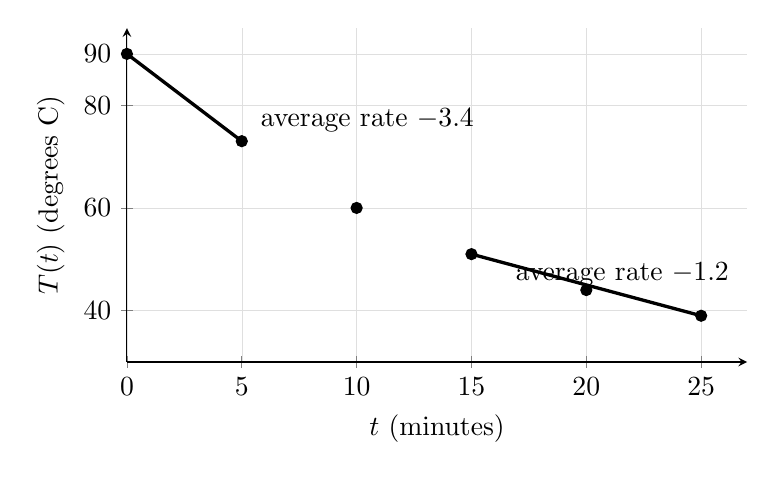
\begin{tikzpicture}
\begin{axis}[
    width=0.78\textwidth,
    height=0.48\textwidth,
    xmin=0, xmax=27,
    ymin=30, ymax=95,
    axis lines=left,
    xlabel={\(t\) (minutes)},
    ylabel={\(T(t)\) (degrees C)},
    xtick={0,5,10,15,20,25},
    ytick={40,60,80,90},
    grid=both,
    grid style={line width=.1pt, draw=gray!25},
]
\addplot[only marks, mark=*] coordinates {
    (0,90) (5,73) (10,60) (15,51) (20,44) (25,39)
};
\addplot[very thick, domain=0:5, samples=2] {90 - 3.4*x};
\addplot[very thick, domain=15:25, samples=2] {51 - 1.2*(x-15)};
\node[anchor=west] at (axis cs:5.4,77) {average rate \(-3.4\)};
\node[anchor=west] at (axis cs:16.5,47) {average rate \(-1.2\)};
\end{axis}
\end{tikzpicture}
\caption{Average rates from data are secant slopes between measured points.}
\label{fig:coffee-average-rates}
\end{figure}

A table gives only certain points.  We can compute average rates between those points, but we cannot know the exact instantaneous rate from the table alone.  We can estimate it by using nearby data, but the estimate depends on the quality and spacing of the measurements.

\subsection{Units of a rate}
\label{subsec:units-of-rate}

The units of an average rate come from the quotient:

\[
\frac{\text{output units}}{\text{input units}}.
\]

That simple rule prevents many mistakes.

\[
\begin{array}{c|c|c}
\textbf{function} & \textbf{average rate} & \textbf{units} \\ \hline
s(t)=\text{position} & \dfrac{s(b)-s(a)}{b-a} & \text{meters/second} \\[8pt]
T(t)=\text{temperature} & \dfrac{T(b)-T(a)}{b-a} & ^\circ\text{C/minute} \\[8pt]
C(q)=\text{cost} & \dfrac{C(b)-C(a)}{b-a} & \text{dollars/item} \\[8pt]
P(t)=\text{population} & \dfrac{P(b)-P(a)}{b-a} & \text{people/year}
\end{array}
\]

The units also explain the meaning of the sign.

If

\[
\frac{T(5)-T(0)}{5-0}=-3.4,
\]

then the coffee temperature is decreasing by an average of \(3.4^\circ\text{C}\) per minute.

If

\[
\frac{P(2030)-P(2020)}{2030-2020}=15000,
\]

then the population is increasing by an average of \(15{,}000\) people per year.

If

\[
\frac{C(101)-C(100)}{101-100}=8.25,
\]

then producing the \(101\)st item increased the cost by \(8.25\) dollars compared with producing \(100\) items.  This is an average over one item, and in many cost models it is close to what economists call marginal cost.

\begin{quote}
\textbf{Meaning before formulas.}
An average rate of change is always a comparison:

\[
\frac{\text{how much the output changed}}{\text{how much the input changed}}.
\]

The units tell what kind of comparison it is.
\end{quote}

Average rates are useful, but they still describe an interval.  A speedometer does not report the average velocity over the last hour.  It reports what is happening now.

To get that number from position, we must make the interval shrink.

\section{Instantaneous rate of change}
\label{sec:instantaneous-rate-of-change}

Average velocity looks across an interval.  Instantaneous velocity looks at one time.

That sounds impossible at first.  If there is only one time, there is no change in time, and a quotient like

\[
\frac{\text{change in position}}{\text{change in time}}
\]

would have denominator \(0\).

The way out is not to divide by \(0\).  The way out is to divide by a nonzero time change \(h\), and then let \(h\) approach \(0\).

\subsection{Shrinking the time interval}
\label{subsec:shrinking-time-interval}

Let

\[
s(t)=t^2
\]

be position in meters after \(t\) seconds.  We want the velocity at \(t=2\).

The average velocity from \(t=2\) to \(t=2+h\) is

\[
\frac{s(2+h)-s(2)}{(2+h)-2}
=
\frac{s(2+h)-s(2)}{h},
\qquad h\neq0.
\]

Compute:

\[
\frac{s(2+h)-s(2)}{h}
=
\frac{(2+h)^2-4}{h}
=
\frac{4+4h+h^2-4}{h}
=
\frac{4h+h^2}{h}.
\]

Since \(h\neq0\),

\[
\frac{4h+h^2}{h}=4+h.
\]

So the average velocity over the interval from \(2\) to \(2+h\) is

\[
4+h.
\]

Now let \(h\) get close to \(0\):

\[
\begin{array}{c|cccccc}
h & -0.1 & -0.01 & -0.001 & 0.001 & 0.01 & 0.1 \\ \hline
4+h & 3.9 & 3.99 & 3.999 & 4.001 & 4.01 & 4.1
\end{array}
\]

The average velocities approach \(4\).  Therefore the instantaneous velocity at \(t=2\) is

\[
4\text{ meters/second}.
\]

The calculation is short, but it carries the central idea:

\[
\text{instantaneous rate}=
\lim_{\text{interval width}\to0}
\text{average rate}.
\]

\subsection{The derivative at a point}
\label{subsec:derivative-at-a-point}

Now we name the limiting average rate.

\begin{quote}
\textbf{Derivative at a point.}
Let \(f\) be a function defined at \(a\) and near \(a\).  The derivative of \(f\) at \(a\), written \(f'(a)\), is

\[
\boxed{
f'(a)=\lim_{h\to0}\frac{f(a+h)-f(a)}{h},
}
\]

provided this limit exists as a finite number.

If the limit exists, we say that \(f\) is \emph{differentiable at \(a\)}.
\end{quote}

The quotient

\[
\frac{f(a+h)-f(a)}{h}
\]

is the average rate of change from \(a\) to \(a+h\).  The derivative is the limit of these average rates as the second point moves toward the first.

There is another form of the same definition.  Put

\[
x=a+h.
\]

Then

\[
h=x-a.
\]

As \(h\to0\), we have \(x\to a\).  The quotient becomes

\[
\frac{f(x)-f(a)}{x-a}.
\]

So

\[
\boxed{
f'(a)=\lim_{x\to a}\frac{f(x)-f(a)}{x-a},
}
\]

when the limit exists.

The two formulas are the same idea written with different variables.

\paragraph{Example: derivative of \(x^2\) at \(2\).}
Let

\[
f(x)=x^2.
\]

Then

\[
f'(2)
=
\lim_{h\to0}\frac{f(2+h)-f(2)}{h}.
\]

We already computed the quotient:

\[
\frac{f(2+h)-f(2)}{h}
=
4+h,
\qquad h\neq0.
\]

Therefore

\[
f'(2)
=
\lim_{h\to0}(4+h)
=
4.
\]

The derivative says that near \(x=2\), the function \(x^2\) is changing at about \(4\) output units per input unit.

\paragraph{Example: derivative of \(x^3\) at \(2\).}
Let

\[
f(x)=x^3.
\]

Then

\[
f'(2)
=
\lim_{h\to0}\frac{(2+h)^3-2^3}{h}.
\]

Expand:

\[
(2+h)^3
=
8+12h+6h^2+h^3.
\]

Thus

\[
\frac{(2+h)^3-8}{h}
=
\frac{12h+6h^2+h^3}{h}.
\]

Since \(h\neq0\),

\[
\frac{12h+6h^2+h^3}{h}
=
12+6h+h^2.
\]

Now take the limit:

\[
f'(2)
=
\lim_{h\to0}(12+6h+h^2)
=
12.
\]

So the instantaneous rate of change of \(x^3\) at \(x=2\) is \(12\).

\paragraph{Example: derivative of \(1/x\) at \(1\).}
Let

\[
f(x)=\frac1x.
\]

Find \(f'(1)\).

\[
f'(1)
=
\lim_{h\to0}\frac{f(1+h)-f(1)}{h}
=
\lim_{h\to0}\frac{\frac{1}{1+h}-1}{h}.
\]

Simplify the numerator:

\[
\frac{1}{1+h}-1
=
\frac{1-(1+h)}{1+h}
=
\frac{-h}{1+h}.
\]

Therefore

\[
\frac{\frac{1}{1+h}-1}{h}
=
\frac{-h}{h(1+h)}.
\]

Since \(h\neq0\),

\[
\frac{-h}{h(1+h)}
=
-\frac{1}{1+h}.
\]

So

\[
f'(1)
=
\lim_{h\to0}\left(-\frac{1}{1+h}\right)
=
-1.
\]

The negative sign matches the graph: \(1/x\) is decreasing near \(x=1\).

\subsection{Tangent slope}
\label{subsec:tangent-slope}

The derivative has a geometric meaning.  It is the slope of the tangent line.

For a curve \(y=f(x)\), the secant line through

\[
(a,f(a))
\qquad\text{and}\qquad
(a+h,f(a+h))
\]

has slope

\[
\frac{f(a+h)-f(a)}{h}.
\]

As \(h\to0\), the second point approaches the first.  If the secant slopes approach a single number, that number is the slope of the tangent line at \((a,f(a))\).

\begin{figure}[h]
\centering
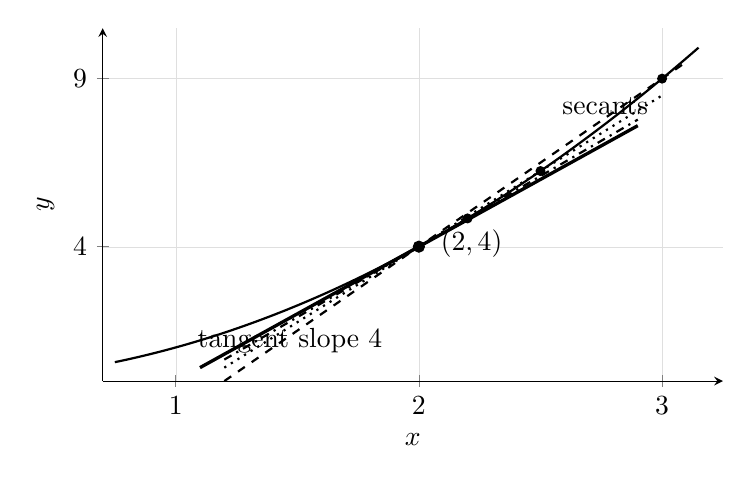
\begin{tikzpicture}
\begin{axis}[
    width=0.78\textwidth,
    height=0.50\textwidth,
    xmin=0.7, xmax=3.25,
    ymin=0, ymax=10.5,
    axis lines=left,
    xlabel={\(x\)},
    ylabel={\(y\)},
    xtick={1,2,3},
    ytick={4,9},
    grid=both,
    grid style={line width=.1pt, draw=gray!25},
]
\addplot[thick, domain=0.75:3.15, samples=100] {x^2};

% secant lines through (2,4) with h=1, 0.5, 0.2
\addplot[thick, dashed, domain=1.2:3.1, samples=2] {5*x-6};
\addplot[thick, dotted, domain=1.2:3.0, samples=2] {4.5*x-5};
\addplot[thick, dashdotted, domain=1.2:2.9, samples=2] {4.2*x-4.4};

% tangent line
\addplot[very thick, domain=1.1:2.9, samples=2] {4*x-4};

\addplot[only marks, mark=*] coordinates {(2,4)};
\addplot[only marks, mark=*, mark size=1.6pt] coordinates {(3,9) (2.5,6.25) (2.2,4.84)};

\node[anchor=west] at (axis cs:2.05,4.1) {\((2,4)\)};
\node[anchor=west] at (axis cs:2.55,8.2) {secants};
\node[anchor=west] at (axis cs:1.05,1.2) {tangent slope \(4\)};
\end{axis}
\end{tikzpicture}
\caption{Secant slopes approach the tangent slope as the second point approaches the first.}
\label{fig:secants-to-tangent-derivative}
\end{figure}

For \(f(x)=x^2\) at \(x=2\), we found

\[
f'(2)=4.
\]

So the tangent line at \((2,4)\) has slope \(4\).  Its equation is

\[
y-4=4(x-2).
\]

Equivalently,

\[
y=4x-4.
\]

This line is not merely drawn to touch the curve.  It is the limiting position of secant lines.

\paragraph{A tangent line can cross the curve.}
It is tempting to say that a tangent line is a line that touches the graph at one point and does not cross it.  That picture works for some curves, but it is not a definition.

For example, let

\[
f(x)=x^3.
\]

At \(x=0\),

\[
f'(0)
=
\lim_{h\to0}\frac{h^3-0}{h}
=
\lim_{h\to0}h^2
=
0.
\]

So the tangent line at \((0,0)\) is

\[
y=0.
\]

But the graph of \(y=x^3\) crosses this line at the origin.  The tangent line is still correct because its slope is the limiting secant slope.

\begin{figure}[h]
\centering
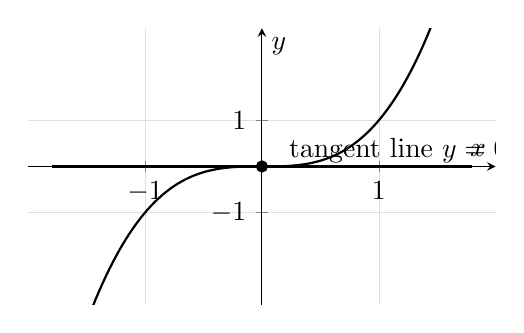
\begin{tikzpicture}
\begin{axis}[
    width=0.62\textwidth,
    height=0.42\textwidth,
    xmin=-2, xmax=2,
    ymin=-3, ymax=3,
    axis lines=middle,
    xlabel={\(x\)},
    ylabel={\(y\)},
    xtick={-1,0,1},
    ytick={-1,0,1},
    grid=both,
    grid style={line width=.1pt, draw=gray!25},
]
\addplot[thick, domain=-1.45:1.45, samples=100] {x^3};
\addplot[very thick, domain=-1.8:1.8, samples=2] {0};
\addplot[only marks, mark=*] coordinates {(0,0)};
\node[anchor=west] at (axis cs:0.15,0.35) {tangent line \(y=0\)};
\end{axis}
\end{tikzpicture}
\caption{A tangent line can cross the curve.  Tangency is about limiting slope, not merely touching.}
\label{fig:cubic-tangent-crosses}
\end{figure}

\subsection{The derivative as a limit}
\label{subsec:derivative-as-limit}

The derivative is a limit of slopes:

\[
f'(a)
=
\lim_{h\to0}
\frac{f(a+h)-f(a)}{h}.
\]

This formula has three layers.

First, the quotient

\[
\frac{f(a+h)-f(a)}{h}
\]

is an average rate of change over an interval.

Second, the limit

\[
h\to0
\]

shrinks the interval toward a single input.

Third, the result \(f'(a)\), if it exists, is the instantaneous rate of change at \(a\).

\[
\boxed{
\text{derivative}
=
\text{limit of average rates}.
}
\]

The limit must exist as one finite number.  If the slopes approach different values from different sides, there is no derivative.

\paragraph{Warning example: the corner in \(|x|\).}
Let

\[
f(x)=|x|.
\]

Try to find \(f'(0)\).

By definition,

\[
f'(0)
=
\lim_{h\to0}\frac{|0+h|-|0|}{h}
=
\lim_{h\to0}\frac{|h|}{h}.
\]

If \(h>0\), then \(|h|=h\), so

\[
\frac{|h|}{h}=1.
\]

If \(h<0\), then \(|h|=-h\), so

\[
\frac{|h|}{h}=-1.
\]

The right-side slopes approach \(1\).  The left-side slopes approach \(-1\).  There is no single limiting slope.

Therefore

\[
f'(0)
\]

does not exist.

\begin{figure}[h]
\centering
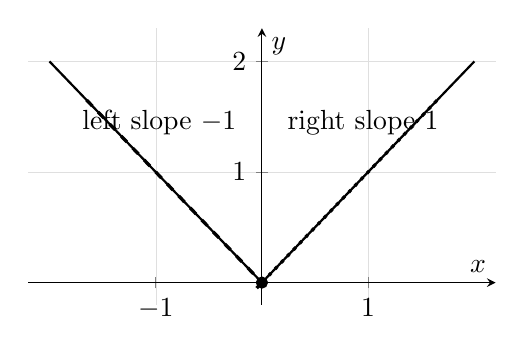
\begin{tikzpicture}
\begin{axis}[
    width=0.62\textwidth,
    height=0.42\textwidth,
    xmin=-2.2, xmax=2.2,
    ymin=-0.2, ymax=2.3,
    axis lines=middle,
    xlabel={\(x\)},
    ylabel={\(y\)},
    xtick={-1,0,1},
    ytick={1,2},
    grid=both,
    grid style={line width=.1pt, draw=gray!25},
]
\addplot[thick, domain=-2:0, samples=2] {-x};
\addplot[thick, domain=0:2, samples=2] {x};
\addplot[very thick, dashed, domain=-1.65:0.05, samples=2] {-x};
\addplot[very thick, dotted, domain=-0.05:1.65, samples=2] {x};
\addplot[only marks, mark=*] coordinates {(0,0)};
\node[anchor=east] at (axis cs:-0.15,1.45) {left slope \(-1\)};
\node[anchor=west] at (axis cs:0.15,1.45) {right slope \(1\)};
\end{axis}
\end{tikzpicture}
\caption{At a corner, the left and right limiting slopes can disagree.  Then the derivative does not exist.}
\label{fig:absolute-value-no-derivative}
\end{figure}

The graph has a sharp corner at the origin.  The corner is not the real reason the derivative fails; it is the picture of the reason.  The reason is that the limiting slopes do not approach one common value.

\begin{quote}
\textbf{What can go wrong?}
The derivative at \(a\) exists only when

\[
\lim_{h\to0}\frac{f(a+h)-f(a)}{h}
\]

exists as a finite number.

If the left and right slopes disagree, or if the slopes grow without bound, then \(f'(a)\) does not exist.
\end{quote}

One derivative gives one slope at one point.  But a curve has many points.  If we let the point \(a\) move, the derivative itself becomes a new function.  That new function will tell us how the whole graph is changing.
\section{The derivative as a function}
\label{sec:derivative-as-function}

Section \ref{sec:instantaneous-rate-of-change} gave the derivative at one point.  For example,

\[
f(x)=x^2
\]

has

\[
f'(2)=4.
\]

That number is the slope of one tangent line.  But a curve has many points, and the slope usually changes from point to point.  If the point moves, the derivative moves with it.

So the derivative is not only a number.  It is also a new function.

\subsection{From one tangent slope to many}
\label{subsec:one-slope-to-many}

The calculation for \(f(x)=x^2\) at \(x=2\) did not really depend on the number \(2\).  Let us repeat it at a general point \(a\).

Let

\[
f(x)=x^2.
\]

Then

\[
f'(a)
=
\lim_{h\to0}\frac{f(a+h)-f(a)}{h}.
\]

Substitute the formula:

\[
f'(a)
=
\lim_{h\to0}\frac{(a+h)^2-a^2}{h}.
\]

Expand:

\[
(a+h)^2=a^2+2ah+h^2.
\]

Therefore

\[
\frac{(a+h)^2-a^2}{h}
=
\frac{2ah+h^2}{h}.
\]

Since \(h\neq0\),

\[
\frac{2ah+h^2}{h}=2a+h.
\]

Now take the limit:

\[
f'(a)=\lim_{h\to0}(2a+h)=2a.
\]

So the tangent slope at \(x=a\) is

\[
2a.
\]

If we let the input point be called \(x\), we write

\[
\boxed{f'(x)=2x.}
\]

This new function \(f'\) gives the slope of the graph of \(f\) at each point where the derivative exists.

\[
\begin{array}{c|ccccc}
x & -2 & -1 & 0 & 1 & 2 \\ \hline
f(x)=x^2 & 4 & 1 & 0 & 1 & 4 \\
f'(x)=2x & -4 & -2 & 0 & 2 & 4
\end{array}
\]

The original function \(f(x)=x^2\) gives heights.  The derivative function \(f'(x)=2x\) gives slopes.

\begin{figure}[h]
\centering
\begin{minipage}{0.48\textwidth}
\centering
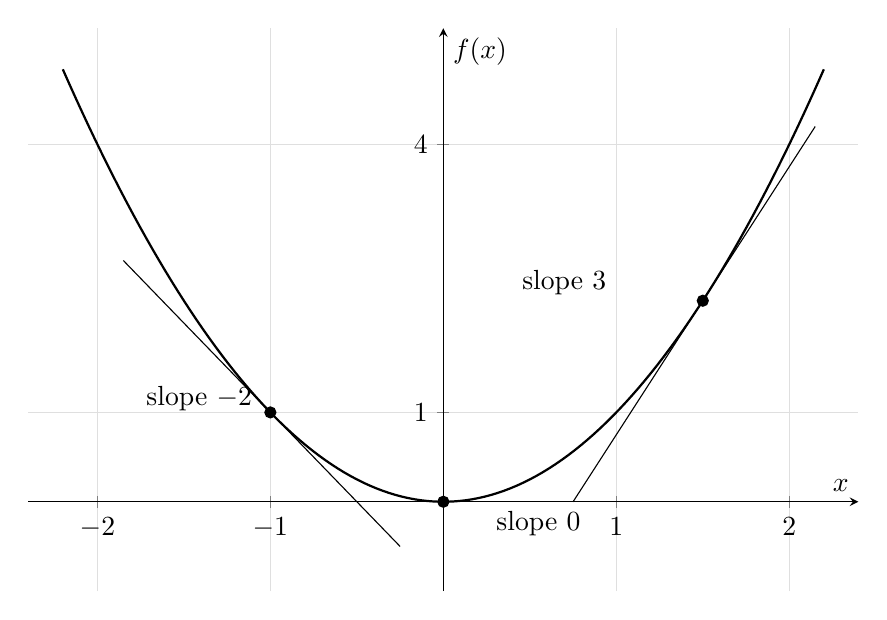
\begin{tikzpicture}
\begin{axis}[
    width=\textwidth,
    height=0.72\textwidth,
    xmin=-2.4, xmax=2.4,
    ymin=-1, ymax=5.3,
    axis lines=middle,
    xlabel={\(x\)},
    ylabel={\(f(x)\)},
    xtick={-2,-1,0,1,2},
    ytick={0,1,4},
    grid=both,
    grid style={line width=.1pt, draw=gray!25},
]
\addplot[thick, domain=-2.2:2.2, samples=120] {x^2};

% Tangent lines
\addplot[thin, domain=-1.85:-0.25, samples=2] {-2*x-1};
\addplot[thin, domain=-0.9:0.9, samples=2] {0};
\addplot[thin, domain=0.75:2.15, samples=2] {3*x-2.25};

\addplot[only marks, mark=*] coordinates {(-1,1) (0,0) (1.5,2.25)};
\node[anchor=east] at (axis cs:-1.05,1.15) {slope \(-2\)};
\node[anchor=north] at (axis cs:0.55,0) {slope \(0\)};
\node[anchor=west] at (axis cs:0.4,2.45) {slope \(3\)};
\end{axis}
\end{tikzpicture}
\end{minipage}
\hfill
\begin{minipage}{0.48\textwidth}
\centering
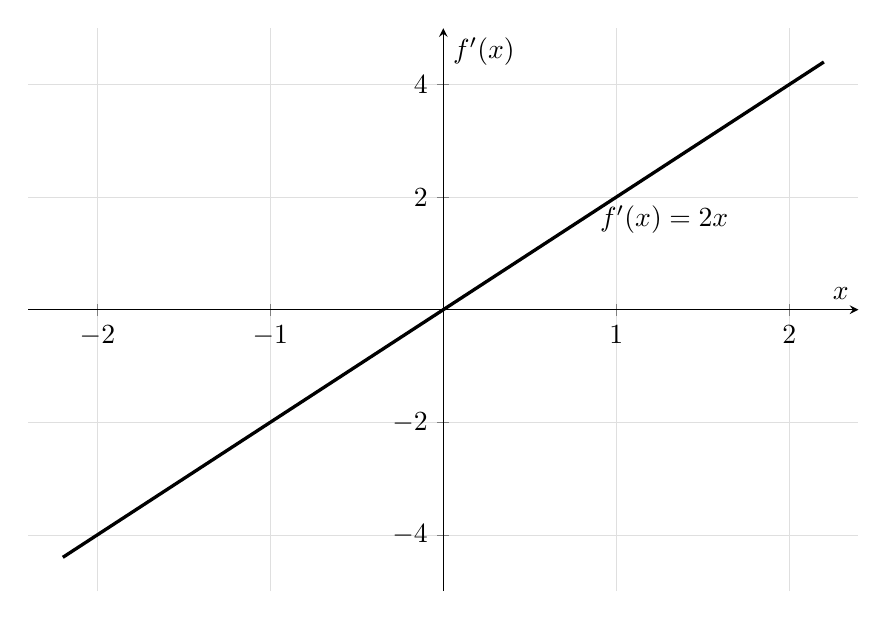
\begin{tikzpicture}
\begin{axis}[
    width=\textwidth,
    height=0.72\textwidth,
    xmin=-2.4, xmax=2.4,
    ymin=-5, ymax=5,
    axis lines=middle,
    xlabel={\(x\)},
    ylabel={\(f'(x)\)},
    xtick={-2,-1,0,1,2},
    ytick={-4,-2,0,2,4},
    grid=both,
    grid style={line width=.1pt, draw=gray!25},
]
\addplot[very thick, domain=-2.2:2.2, samples=2] {2*x};
\node[anchor=west] at (axis cs:0.85,1.6) {\(f'(x)=2x\)};
\end{axis}
\end{tikzpicture}
\end{minipage}
\caption{The graph of \(f\) shows height.  The graph of \(f'\) shows tangent slope.}
\label{fig:parabola-and-derivative}
\end{figure}

\begin{quote}
\textbf{Derivative function.}
The derivative function of \(f\) is

\[
\boxed{
f'(x)=\lim_{h\to0}\frac{f(x+h)-f(x)}{h},
}
\]

defined at every \(x\) where this limit exists.
\end{quote}

The domain of \(f'\) may be smaller than the domain of \(f\).  For example,

\[
f(x)=|x|
\]

is defined for every real number \(x\).  But at \(x=0\),

\[
\lim_{h\to0}\frac{|h|}{h}
\]

does not exist, because the left and right limiting slopes disagree.  For \(x<0\), the graph is the line \(y=-x\), so the slope is \(-1\).  For \(x>0\), the graph is the line \(y=x\), so the slope is \(1\).  Thus

\[
f'(x)=
\begin{cases}
-1, & x<0,\\
1, & x>0,
\end{cases}
\]

and \(f'(0)\) does not exist.

A derivative function records where slopes exist.  It also records where they fail to exist.

\paragraph{Example: the derivative function of \(x^3\).}
Let

\[
f(x)=x^3.
\]

Then

\[
f'(x)
=
\lim_{h\to0}\frac{(x+h)^3-x^3}{h}.
\]

Expand:

\[
(x+h)^3=x^3+3x^2h+3xh^2+h^3.
\]

So

\[
\frac{(x+h)^3-x^3}{h}
=
\frac{3x^2h+3xh^2+h^3}{h}.
\]

Since \(h\neq0\),

\[
\frac{3x^2h+3xh^2+h^3}{h}
=
3x^2+3xh+h^2.
\]

Therefore

\[
f'(x)
=
\lim_{h\to0}(3x^2+3xh+h^2)
=
3x^2.
\]

So

\[
\boxed{\frac{d}{dx}x^3=3x^2.}
\]

At \(x=0\), this derivative is \(0\), so the tangent line to \(y=x^3\) at the origin is horizontal.  But the graph crosses the tangent line there.  Again, the derivative is about limiting slope, not about merely touching.

\subsection{Notations for the derivative}
\label{subsec:derivative-notations}

The derivative is important enough to have several notations.  Each notation emphasizes a different part of the same idea.

If

\[
y=f(x),
\]

then the following notations all refer to the derivative:

\[
\begin{array}{c|l}
\textbf{notation} & \textbf{meaning} \\ \hline
f'(x) & \text{the derivative function of }f \\[3pt]
\dfrac{dy}{dx} & \text{the rate of change of }y\text{ with respect to }x \\[8pt]
\dfrac{d}{dx}f(x) & \text{the result of differentiating }f(x)\text{ with respect to }x \\[8pt]
D_x f(x) & \text{another compact notation for the same operation}
\end{array}
\]

For example, if

\[
y=x^2,
\]

then

\[
f'(x)=2x,
\]

and we may also write

\[
\frac{dy}{dx}=2x,
\]

or

\[
\frac{d}{dx}(x^2)=2x,
\]

or

\[
D_x(x^2)=2x.
\]

At a particular point \(x=a\), we write

\[
\left.\frac{dy}{dx}\right|_{x=a}=f'(a).
\]

For instance, if \(y=x^2\), then

\[
\left.\frac{dy}{dx}\right|_{x=3}=6.
\]

That means the tangent slope at \(x=3\) is \(6\).

\paragraph{Leibniz notation remembers the units.}
If \(s(t)\) is position in meters and \(t\) is time in seconds, then

\[
\frac{ds}{dt}
\]

has units

\[
\frac{\text{meters}}{\text{seconds}}.
\]

So

\[
v(t)=s'(t)=\frac{ds}{dt}
\]

is velocity.

If \(T(t)\) is temperature in degrees Celsius and \(t\) is time in minutes, then

\[
\frac{dT}{dt}
\]

has units

\[
\frac{^\circ\text{C}}{\text{minute}}.
\]

So \(\dfrac{dT}{dt}\) measures how quickly the temperature is changing.

\begin{quote}
\textbf{A caution about \(\dfrac{dy}{dx}\).}
The notation

\[
\frac{dy}{dx}
\]

comes from the quotient

\[
\frac{\Delta y}{\Delta x}.
\]

At this stage, it means a limit of such quotients.  It is not introduced as an ordinary fraction of two real numbers.

In the next section, \(dx\) and \(dy\) will acquire a useful meaning through linear approximation.
\end{quote}

\subsection{Reading \(f'\) from the graph of \(f\)}
\label{subsec:reading-derivative-from-function-graph}

The graph of \(f\) contains the graph of \(f'\) in hidden form.  At each \(x\), the value \(f'(x)\) is the slope of the tangent line to the graph of \(f\).

This gives several visual rules.

\[
\begin{array}{c|c}
\textbf{feature of }f & \textbf{meaning for }f' \\ \hline
f\text{ is rising} & f'(x)>0 \\[2pt]
f\text{ is falling} & f'(x)<0 \\[2pt]
f\text{ has a horizontal tangent} & f'(x)=0 \\[2pt]
f\text{ is steep} & |f'(x)|\text{ is large} \\[2pt]
f\text{ has a sharp corner} & f'(x)\text{ may not exist}
\end{array}
\]

\paragraph{Example.}
Let

\[
f(x)=x^3-3x.
\]

We compute \(f'(x)\) from the definition.  The difference quotient is

\[
\frac{f(x+h)-f(x)}{h}
=
\frac{(x+h)^3-3(x+h)-(x^3-3x)}{h}.
\]

Simplify the numerator:

\[
(x+h)^3-3(x+h)-(x^3-3x)
=
3x^2h+3xh^2+h^3-3h.
\]

So

\[
\frac{f(x+h)-f(x)}{h}
=
3x^2+3xh+h^2-3.
\]

Taking the limit gives

\[
f'(x)=3x^2-3.
\]

The derivative graph is a graph of slopes.

\begin{figure}[h]
\centering
\begin{minipage}{0.48\textwidth}
\centering
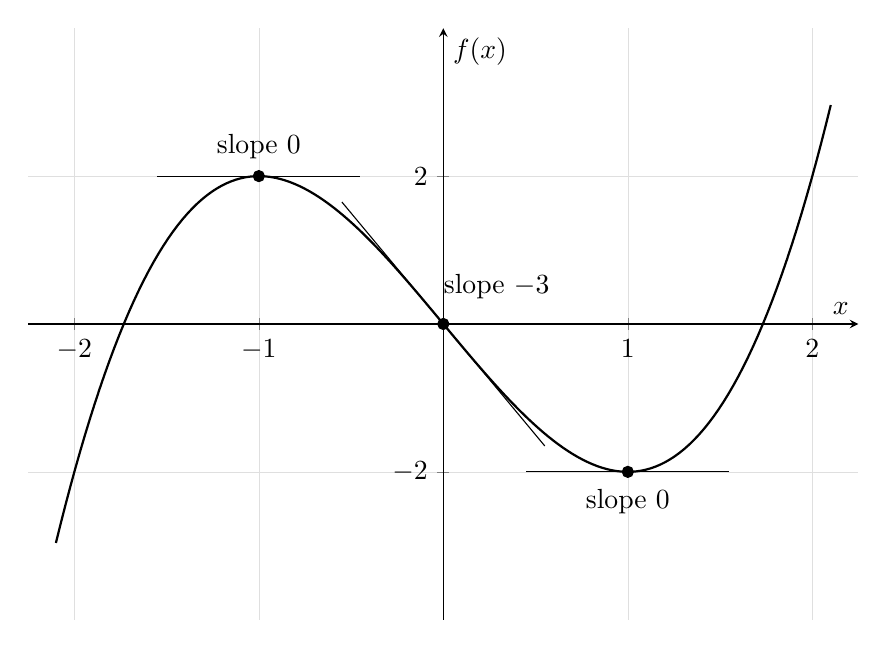
\begin{tikzpicture}
\begin{axis}[
    width=\textwidth,
    height=0.75\textwidth,
    xmin=-2.25, xmax=2.25,
    ymin=-4, ymax=4,
    axis lines=middle,
    xlabel={\(x\)},
    ylabel={\(f(x)\)},
    xtick={-2,-1,0,1,2},
    ytick={-2,0,2},
    grid=both,
    grid style={line width=.1pt, draw=gray!25},
]
\addplot[thick, domain=-2.1:2.1, samples=160] {x^3-3*x};
\addplot[only marks, mark=*] coordinates {(-1,2) (1,-2) (0,0)};
\addplot[thin, domain=-1.55:-0.45, samples=2] {2};
\addplot[thin, domain=0.45:1.55, samples=2] {-2};
\addplot[thin, domain=-0.55:0.55, samples=2] {-3*x};
\node[anchor=south] at (axis cs:-1,2.1) {slope \(0\)};
\node[anchor=north] at (axis cs:1,-2.1) {slope \(0\)};
\node[anchor=west] at (axis cs:-0.05,0.5) {slope \(-3\)};
\end{axis}
\end{tikzpicture}
\end{minipage}
\hfill
\begin{minipage}{0.48\textwidth}
\centering
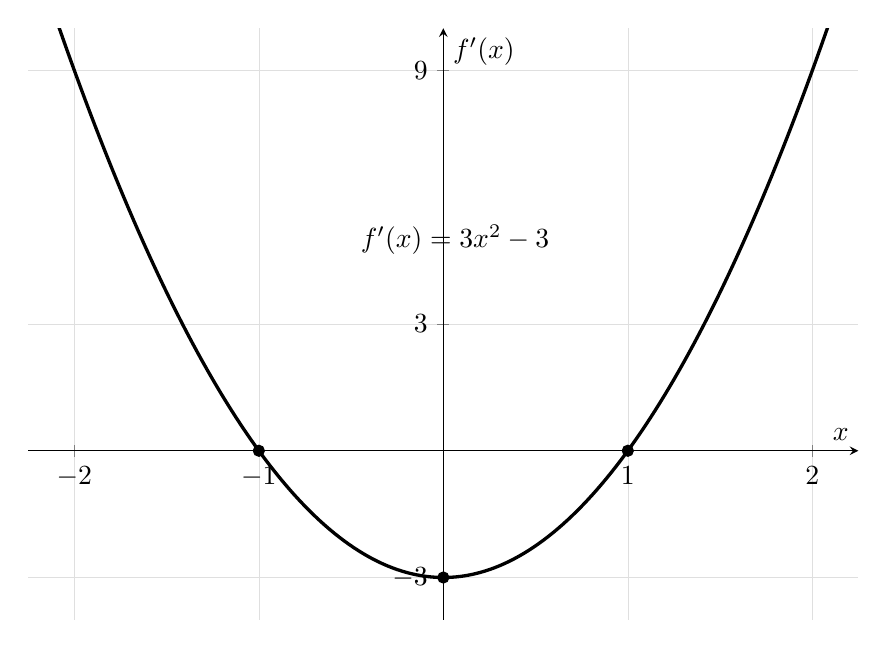
\begin{tikzpicture}
\begin{axis}[
    width=\textwidth,
    height=0.75\textwidth,
    xmin=-2.25, xmax=2.25,
    ymin=-4, ymax=10,
    axis lines=middle,
    xlabel={\(x\)},
    ylabel={\(f'(x)\)},
    xtick={-2,-1,0,1,2},
    ytick={-3,0,3,9},
    grid=both,
    grid style={line width=.1pt, draw=gray!25},
]
\addplot[very thick, domain=-2.1:2.1, samples=160] {3*x^2-3};
\addplot[only marks, mark=*] coordinates {(-1,0) (1,0) (0,-3)};
\node[anchor=west] at (axis cs:-0.5,5) {\(f'(x)=3x^2-3\)};
\end{axis}
\end{tikzpicture}
\end{minipage}
\caption{The derivative graph records the slopes of the original graph.}
\label{fig:cubic-and-derivative}
\end{figure}

The original graph has horizontal tangents at \(x=-1\) and \(x=1\).  The derivative graph has zeros there:

\[
f'(-1)=0,
\qquad
f'(1)=0.
\]

At \(x=0\), the original graph is falling with slope \(-3\).  The derivative graph has value

\[
f'(0)=-3.
\]

The derivative graph does not show the height of \(f\).  It shows how the height is changing.

\subsection{Reading \(f\) from the graph of \(f'\)}
\label{subsec:reading-function-from-derivative-graph}

The derivative graph also gives information in the opposite direction.

If \(f'(x)>0\), then the tangent slopes are positive, so \(f\) is rising.

If \(f'(x)<0\), then the tangent slopes are negative, so \(f\) is falling.

If \(f'(x)=0\), then the graph of \(f\) has a horizontal tangent.

For the example

\[
f'(x)=3x^2-3,
\]

we have

\[
3x^2-3>0
\]

when

\[
x<-1
\qquad\text{or}\qquad
x>1.
\]

So the graph of \(f\) is rising on those intervals.

We also have

\[
3x^2-3<0
\]

when

\[
-1<x<1.
\]

So the graph of \(f\) is falling there.

Thus the derivative graph tells the shape story:

\[
\text{rising} \quad \longrightarrow \quad \text{falling} \quad \longrightarrow \quad \text{rising}.
\]

This is why derivatives help us understand graphs.  A derivative is local information, but when we collect it point by point, it begins to describe the whole curve.

\paragraph{What \(f'\) does not tell by itself.}
The derivative does not remember vertical shifts.

Let

\[
f(x)=x^2
\qquad\text{and}\qquad
g(x)=x^2+5.
\]

For \(f\),

\[
f'(x)=2x.
\]

For \(g\),

\[
g'(x)
=
\lim_{h\to0}\frac{(x+h)^2+5-(x^2+5)}{h}
=
\lim_{h\to0}\frac{(x+h)^2-x^2}{h}
=
2x.
\]

So

\[
f'(x)=g'(x),
\]

even though

\[
g(x)=f(x)+5.
\]

The two graphs have the same slopes at corresponding \(x\)-values, but one graph is \(5\) units higher.

\begin{quote}
\textbf{The derivative forgets constants.}
A derivative records change.  Adding a constant changes height, but not slope.
\end{quote}

This points toward the second half of calculus.  If we know all the slopes \(f'(x)\), how much of \(f\) can we recover?  We will eventually need a starting value and a way to accumulate slope information.

Before that larger question, we use the derivative for a more local purpose: near one point, a curve can be replaced by a line.

\section{Local linear approximation}
\label{sec:local-linear-approximation}

The derivative function records many slopes.  At a single point, the derivative does something even more practical: it gives the best linear model of the function near that point.

A curved graph may be difficult.  A line is simple.  Calculus lets us replace a curve by a line, as long as we stay close enough to the point of tangency.

\subsection{The tangent line as a local model}
\label{subsec:tangent-line-local-model}

Suppose we want to estimate

\[
\sqrt{4.1}
\]

without a calculator.

The nearby value

\[
\sqrt4=2
\]

is easy.  The question is how much \(\sqrt{x}\) changes when \(x\) moves from \(4\) to \(4.1\).

Let

\[
f(x)=\sqrt{x}.
\]

We need the derivative at \(x=4\).  By definition,

\[
f'(4)
=
\lim_{h\to0}\frac{\sqrt{4+h}-2}{h}.
\]

Multiply numerator and denominator by the conjugate:

\[
\frac{\sqrt{4+h}-2}{h}
\cdot
\frac{\sqrt{4+h}+2}{\sqrt{4+h}+2}
=
\frac{(4+h)-4}{h(\sqrt{4+h}+2)}.
\]

So, for \(h\neq0\),

\[
\frac{\sqrt{4+h}-2}{h}
=
\frac{1}{\sqrt{4+h}+2}.
\]

Taking the limit gives

\[
f'(4)=\frac{1}{2+2}=\frac14.
\]

Thus near \(x=4\), the graph of \(y=\sqrt{x}\) has tangent slope \(\frac14\).  The tangent line at \((4,2)\) is

\[
y-2=\frac14(x-4).
\]

So

\[
L(x)=2+\frac14(x-4).
\]

This line is the local linear model of \(\sqrt{x}\) near \(x=4\).

Now plug in \(x=4.1\):

\[
\sqrt{4.1}
\approx
L(4.1)
=
2+\frac14(0.1)
=
2+0.025
=
2.025.
\]

A calculator gives

\[
\sqrt{4.1}\approx2.024845\ldots,
\]

so the tangent-line estimate is very close.

\begin{figure}[h]
\centering
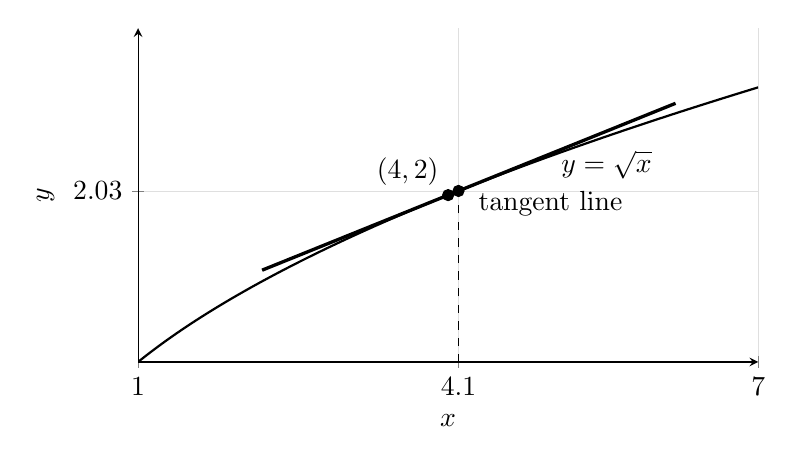
\begin{tikzpicture}
\begin{axis}[
    width=0.78\textwidth,
    height=0.48\textwidth,
    xmin=1, xmax=7,
    ymin=1, ymax=3,
    axis lines=left,
    xlabel={\(x\)},
    ylabel={\(y\)},
    xtick={1,4.1,7},
    xticklabels={\(1\),\(4.1\),\(7\)},
    ytick={2.025},
    grid=both,
    grid style={line width=.1pt, draw=gray!25},
]
\addplot[thick, domain=1:7, samples=160] {sqrt(x)};
\addplot[very thick, domain=2.2:6.2, samples=2] {2 + 0.25*(x-4)};
\addplot[only marks, mark=*] coordinates {(4,2) (4.1,2.0248457)};
\draw[dashed] (axis cs:4.1,0) -- (axis cs:4.1,2.0248457);
\node[anchor=south east] at (axis cs:4,2) {\((4,2)\)};
\node[anchor=west] at (axis cs:4.2,1.95) {tangent line};
\node[anchor=west] at (axis cs:5.0,2.18) {\(y=\sqrt{x}\)};
\end{axis}
\end{tikzpicture}
\caption{Near \(x=4\), the tangent line gives a simple model for \(\sqrt{x}\).}
\label{fig:sqrt-local-linear}
\end{figure}

The tangent line does not equal the curve except at the point of tangency.  But near that point, the line and the curve are close.

\subsection{The formula \(f(a+h)\approx f(a)+f'(a)h\)}
\label{subsec:local-linear-formula}

The square-root example has a general form.

Suppose \(f\) is differentiable at \(a\).  The tangent line at \((a,f(a))\) has slope \(f'(a)\).  Its equation is

\[
y-f(a)=f'(a)(x-a).
\]

So the tangent-line function is

\[
L_a(x)=f(a)+f'(a)(x-a).
\]

This function is called the \emph{linearization} of \(f\) at \(a\).

\begin{quote}
\textbf{Linearization.}
If \(f\) is differentiable at \(a\), then the linearization of \(f\) at \(a\) is

\[
\boxed{
L_a(x)=f(a)+f'(a)(x-a).
}
\]

For \(x\) close to \(a\),

\[
\boxed{
f(x)\approx f(a)+f'(a)(x-a).
}
\]
\end{quote}

It is often cleaner to write

\[
x=a+h.
\]

Then \(h=x-a\), and the approximation becomes

\[
\boxed{
f(a+h)\approx f(a)+f'(a)h.
}
\]

This is the derivative in its most useful form:

\[
\text{new value} \approx \text{old value} + \text{slope}\cdot\text{small change}.
\]

\paragraph{Example.}
Let

\[
f(x)=x^2.
\]

At \(a=3\),

\[
f(3)=9
\]

and

\[
f'(3)=6.
\]

So near \(x=3\),

\[
f(3+h)\approx 9+6h.
\]

If \(h=0.02\), then

\[
(3.02)^2=f(3.02)\approx 9+6(0.02)=9.12.
\]

The exact value is

\[
(3.02)^2=9.1204.
\]

The tangent-line estimate misses by only

\[
0.0004.
\]

The reason is visible from the algebra:

\[
(3+h)^2=9+6h+h^2.
\]

The linear approximation keeps the terms

\[
9+6h
\]

and drops the small term

\[
h^2.
\]

When \(h\) is small, \(h^2\) is much smaller.

\subsection{Why differentiability means local linearity}
\label{subsec:differentiability-local-linearity}

The derivative began as a limit of slopes:

\[
f'(a)=\lim_{h\to0}\frac{f(a+h)-f(a)}{h}.
\]

This says that, for small \(h\),

\[
\frac{f(a+h)-f(a)}{h}
\]

is close to \(f'(a)\).  Multiplying by \(h\), we get the approximation

\[
f(a+h)-f(a)\approx f'(a)h.
\]

So

\[
f(a+h)\approx f(a)+f'(a)h.
\]

There is a precise version.

\begin{quote}
\textbf{Differentiability as local linearity.}
If \(f\) is differentiable at \(a\), then

\[
f(a+h)=f(a)+f'(a)h+E(h),
\]

where the error \(E(h)\) satisfies

\[
\lim_{h\to0}\frac{E(h)}{h}=0.
\]

Equivalently,

\[
\frac{|E(h)|}{|h|}\to0.
\]

So the error is small compared with the size of the input change.
\end{quote}

\paragraph{Proof.}
Define

\[
E(h)=f(a+h)-f(a)-f'(a)h.
\]

Then, for \(h\neq0\),

\[
\frac{E(h)}{h}
=
\frac{f(a+h)-f(a)}{h}-f'(a).
\]

Since

\[
\frac{f(a+h)-f(a)}{h}\to f'(a),
\]

we have

\[
\frac{E(h)}{h}\to0.
\]

That is exactly the claim.

\paragraph{Why the derivative hypothesis matters.}
The function

\[
f(x)=|x|
\]

has no derivative at \(0\).  There is no single line that gives a first-order model of \(|x|\) at the origin.

Suppose we try a line through the origin,

\[
L(h)=mh.
\]

The error would be

\[
E(h)=|h|-mh.
\]

For \(h>0\),

\[
\frac{E(h)}{h}=1-m.
\]

For \(h<0\),

\[
\frac{E(h)}{h}=-1-m.
\]

For both one-sided errors to approach \(0\), we would need

\[
1-m=0
\]

and

\[
-1-m=0.
\]

That would require

\[
m=1
\qquad\text{and}\qquad
m=-1
\]

at the same time.  Impossible.

So \(|x|\) has no local linear approximation at \(0\) with error small compared to \(h\).  This is the algebraic meaning of the corner.

\subsection{Differentials}
\label{subsec:differentials}

The notation \(\dfrac{dy}{dx}\) suggests small changes in \(x\) and \(y\).  Linear approximation lets us give that suggestion a precise first meaning.

Let

\[
y=f(x).
\]

Suppose the input changes by a small amount

\[
\Delta x.
\]

Then the exact change in output is

\[
\Delta y=f(x+\Delta x)-f(x).
\]

The derivative gives the tangent-line estimate

\[
\Delta y\approx f'(x)\Delta x.
\]

We now introduce differential notation:

\[
dx=\Delta x,
\]

and

\[
\boxed{
dy=f'(x)\,dx.
}
\]

Here \(dy\) is not the exact change in \(y\).  It is the change predicted by the tangent line.

\[
\boxed{
\Delta y=\text{exact change},
\qquad
dy=\text{linear approximation to the change}.
}
\]

\begin{figure}[h]
\centering
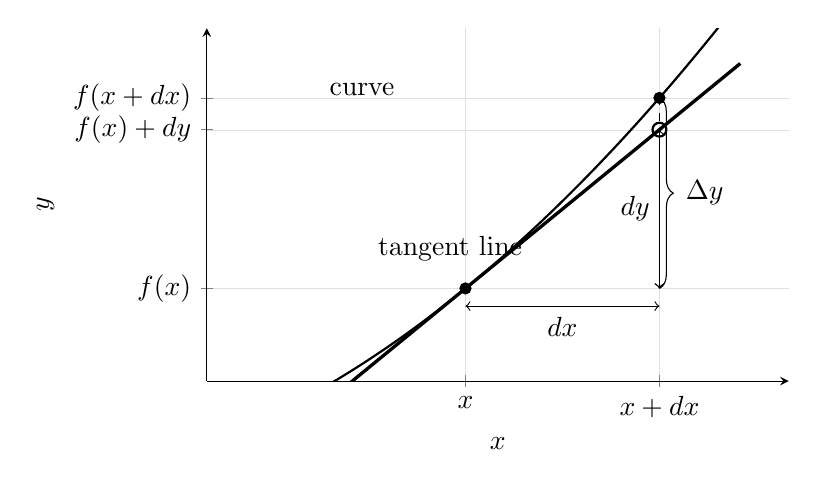
\begin{tikzpicture}
\begin{axis}[
    width=0.74\textwidth,
    height=0.50\textwidth,
    xmin=0.7, xmax=2.5,
    ymin=1.2, ymax=5.2,
    axis lines=left,
    xlabel={\(x\)},
    ylabel={\(y\)},
    xtick={1.5,2.1},
    xticklabels={\(x\),\(x+dx\)},
    ytick={2.25,4.05,4.41},
    yticklabels={\(f(x)\),\(f(x)+dy\),\(f(x+dx)\)},
    grid=both,
    grid style={line width=.1pt, draw=gray!25},
]
\addplot[thick, domain=0.8:2.35, samples=120] {x^2};
\addplot[very thick, domain=1.0:2.35, samples=2] {3*x-2.25};

\addplot[only marks, mark=*] coordinates {(1.5,2.25) (2.1,4.41)};
\addplot[only marks, mark=o, mark size=2.5pt, thick] coordinates {(2.1,4.05)};

\draw[<->] (axis cs:1.5,2.05) -- (axis cs:2.1,2.05);
\node[anchor=north] at (axis cs:1.8,2.03) {\(dx\)};

\draw[<->] (axis cs:2.1,2.25) -- (axis cs:2.1,4.05);
\node[anchor=east] at (axis cs:2.1,3.15) {\(dy\)};

\draw[<->, dashed] (axis cs:2.1,2.25) -- (axis cs:2.1,4.41);
\draw[decorate, decoration={brace, mirror, amplitude=5pt}] 
    (axis cs:2.1,2.25) -- (axis cs:2.1,4.41) 
    node[midway, right=6pt] {\(\Delta y\)};

\node[anchor=west] at (axis cs:1.2,2.7) {tangent line};
\node[anchor=west] at (axis cs:1.05,4.5) {curve};
\end{axis}
\end{tikzpicture}
\caption{The differential \(dy\) is the tangent-line change.  The actual change is \(\Delta y\).}
\label{fig:dy-vs-delta-y}
\end{figure}

\paragraph{Example.}
Let

\[
y=x^2.
\]

Then

\[
\frac{dy}{dx}=2x,
\]

so

\[
dy=2x\,dx.
\]

At \(x=3\), if

\[
dx=0.02,
\]

then

\[
dy=2(3)(0.02)=0.12.
\]

The exact change is

\[
\Delta y=(3.02)^2-3^2=9.1204-9=0.1204.
\]

So the differential estimate is close:

\[
dy=0.12,
\qquad
\Delta y=0.1204.
\]

If instead

\[
dx=-0.02,
\]

then

\[
dy=2(3)(-0.02)=-0.12.
\]

The exact change is

\[
\Delta y=(2.98)^2-9=8.8804-9=-0.1196.
\]

The sign matters.  A positive \(dx\) moves to the right.  A negative \(dx\) moves to the left.  The differential notation remembers the direction of the small step.

\begin{quote}
\textbf{Differential approximation.}
For small \(dx\),

\[
\boxed{
\Delta y\approx dy=f'(x)\,dx.
}
\]

This is the same idea as

\[
f(x+dx)\approx f(x)+f'(x)\,dx.
\]
\end{quote}

\subsection{Sensitivity and propagated error}
\label{subsec:sensitivity-propagated-error}

A derivative measures sensitivity.  If \(x\) has a small error \(dx\), then the resulting error in \(y=f(x)\) is approximately

\[
dy=f'(x)\,dx.
\]

The larger \(|f'(x)|\) is, the more sensitive the output is to small input changes.

\paragraph{Example: measuring the area of a circle.}
The area of a circle of radius \(r\) is

\[
A(r)=\pi r^2.
\]

Since the derivative of \(r^2\) is \(2r\),

\[
A'(r)=2\pi r.
\]

Therefore

\[
dA=2\pi r\,dr.
\]

Suppose the radius is measured as

\[
r=10\text{ cm},
\]

with possible error

\[
|dr|\le0.05\text{ cm}.
\]

Then the approximate area error is bounded by

\[
|dA|
\approx
2\pi(10)(0.05)
=
\pi.
\]

So the area is uncertain by about

\[
\pi\text{ cm}^2.
\]

The relative error is also easy to estimate:

\[
\frac{dA}{A}
=
\frac{2\pi r\,dr}{\pi r^2}
=
2\frac{dr}{r}.
\]

With \(r=10\) and \(|dr|\le0.05\),

\[
\left|\frac{dA}{A}\right|
\approx
2\frac{0.05}{10}
=
0.01.
\]

So the radius error of about \(0.5\%\) produces an area error of about \(1\%\).

\paragraph{Example: sensitivity near division by zero.}
Let

\[
R(x)=\frac1x.
\]

For \(x\neq0\),

\[
R'(x)
=
\lim_{h\to0}\frac{\frac1{x+h}-\frac1x}{h}.
\]

Simplify:

\[
\frac{\frac1{x+h}-\frac1x}{h}
=
\frac{\frac{x-(x+h)}{x(x+h)}}{h}
=
\frac{-h}{h\,x(x+h)}.
\]

Since \(h\neq0\),

\[
\frac{-h}{h\,x(x+h)}
=
-\frac{1}{x(x+h)}.
\]

Taking the limit gives

\[
R'(x)=-\frac1{x^2}.
\]

Near \(x=0\), this derivative is large in magnitude.  For example, at

\[
x=0.01,
\]

we have

\[
R'(0.01)=-\frac{1}{(0.01)^2}=-10000.
\]

A tiny input change

\[
dx=0.0001
\]

produces the approximate output change

\[
dR\approx -10000(0.0001)=-1.
\]

So near \(0\), the reciprocal function is extremely sensitive.  This is the same warning we saw in limits: small denominators can make small input errors become large output errors.

\begin{quote}
\textbf{Sensitivity rule.}
For small input changes,

\[
\boxed{
\text{output change}\approx f'(x)\cdot \text{input change}.
}
\]

The derivative is the local conversion factor from input error to output error.
\end{quote}

Local linear approximation is one of the main reasons derivatives matter.  A differentiable function may be curved, but under enough magnification it behaves like a line.

That raises the next question.  If a function has a derivative at a point, what does that force the original function to do near that point?  In particular, can a differentiable function jump?  The answer is no, and the reason is hidden inside the same local linear formula.
\section{Differentiability and continuity}
\label{sec:differentiability-continuity}

Local linear approximation ended with the formula

\[
f(a+h)=f(a)+f'(a)h+E(h),
\qquad
\frac{E(h)}{h}\to0.
\]

This says that, near \(a\), a differentiable function behaves like a line.  A line cannot jump.  So a differentiable function cannot jump either.

That is our first structural theorem about derivatives:

\[
\text{differentiability is stronger than continuity.}
\]

\subsection{Differentiability implies continuity}
\label{subsec:differentiability-implies-continuity}

Recall what continuity at \(a\) means:

\[
\lim_{x\to a}f(x)=f(a).
\]

In the \(h\)-notation, where \(x=a+h\), this is

\[
\lim_{h\to0}f(a+h)=f(a).
\]

So continuity says that small input changes produce small output changes.  Differentiability says more: small input changes produce output changes that are nearly linear.

\paragraph{A first example.}
Let

\[
f(x)=x^2.
\]

At \(a=3\),

\[
f(3+h)=(3+h)^2=9+6h+h^2.
\]

So

\[
f(3+h)-f(3)=6h+h^2.
\]

As \(h\to0\),

\[
6h+h^2\to0.
\]

Therefore

\[
f(3+h)\to f(3).
\]

The derivative at \(3\) is \(6\), but continuity only needs the weaker fact that the output change goes to \(0\).

The same idea works for every differentiable function.

\begin{quote}
\textbf{Theorem.}
If \(f\) is differentiable at \(a\), then \(f\) is continuous at \(a\).
\end{quote}

\paragraph{Proof.}
Since \(f\) is differentiable at \(a\), the limit

\[
f'(a)=\lim_{h\to0}\frac{f(a+h)-f(a)}{h}
\]

exists as a finite number.

For \(h\neq0\), write

\[
f(a+h)-f(a)
=
h\cdot \frac{f(a+h)-f(a)}{h}.
\]

Now let \(h\to0\).  The first factor \(h\) approaches \(0\).  The second factor approaches the finite number \(f'(a)\).  Therefore the product approaches

\[
0\cdot f'(a)=0.
\]

Thus

\[
\lim_{h\to0}\bigl(f(a+h)-f(a)\bigr)=0.
\]

So

\[
\lim_{h\to0}f(a+h)=f(a).
\]

That is exactly continuity at \(a\).

\[
\boxed{
\text{differentiable at }a
\quad \Longrightarrow \quad
\text{continuous at }a.
}
\]

The proof is short because the idea is simple.  If

\[
\frac{\text{output change}}{\text{input change}}
\]

settles to a finite number, then the output change itself must go to \(0\) when the input change goes to \(0\).

\subsection{Why the converse is false}
\label{subsec:continuity-not-differentiability}

The theorem has only one direction.  Differentiability implies continuity, but continuity does not imply differentiability.

Continuity says the graph has no break at the point.  Differentiability says the graph has one limiting slope there.  A graph can be unbroken and still have no single tangent slope.

The first warning example is

\[
f(x)=|x|.
\]

This function is continuous at \(0\), because

\[
\lim_{x\to0}|x|=0=|0|.
\]

But the derivative at \(0\) would be

\[
f'(0)=\lim_{h\to0}\frac{|h|-0}{h}
=
\lim_{h\to0}\frac{|h|}{h}.
\]

If \(h>0\), then

\[
\frac{|h|}{h}=1.
\]

If \(h<0\), then

\[
\frac{|h|}{h}=-1.
\]

The right-hand slopes approach \(1\).  The left-hand slopes approach \(-1\).  There is no single limiting slope.

Therefore

\[
f'(0)
\]

does not exist.

\[
\boxed{
|x|\text{ is continuous at }0,\text{ but not differentiable at }0.
}
\]

The graph does not jump.  It turns too sharply.

\begin{figure}[h]
\centering
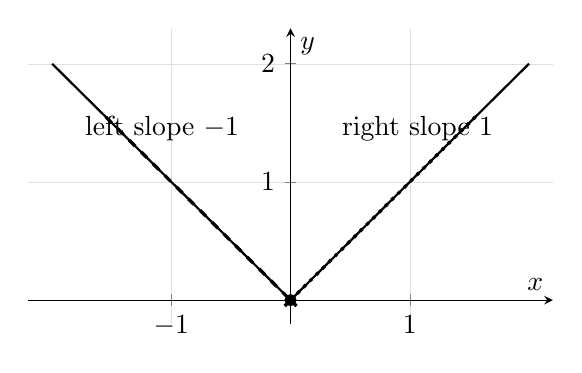
\begin{tikzpicture}
\begin{axis}[
    width=0.68\textwidth,
    height=0.44\textwidth,
    xmin=-2.2, xmax=2.2,
    ymin=-0.2, ymax=2.3,
    axis lines=middle,
    xlabel={\(x\)},
    ylabel={\(y\)},
    xtick={-1,0,1},
    ytick={1,2},
    grid=both,
    grid style={line width=.1pt, draw=gray!25},
]
\addplot[thick, domain=-2:0, samples=2] {-x};
\addplot[thick, domain=0:2, samples=2] {x};
\addplot[very thick, dashed, domain=-1.55:0.05, samples=2] {-x};
\addplot[very thick, dotted, domain=-0.05:1.55, samples=2] {x};
\addplot[only marks, mark=*] coordinates {(0,0)};
\node[anchor=east] at (axis cs:-0.35,1.45) {left slope \(-1\)};
\node[anchor=west] at (axis cs:0.35,1.45) {right slope \(1\)};
\end{axis}
\end{tikzpicture}
\caption{The graph of \(y=|x|\) is continuous at \(0\), but the two limiting slopes disagree.}
\label{fig:absolute-value-continuous-not-differentiable}
\end{figure}

This example separates two ideas that are easy to confuse:

\[
\text{continuity is about nearby heights,}
\]

while

\[
\text{differentiability is about nearby slopes.}
\]

\subsection{Corners, cusps, vertical tangents, and jumps}
\label{subsec:ways-differentiability-can-fail}

The derivative at \(a\) exists only if the difference quotient

\[
\frac{f(a+h)-f(a)}{h}
\]

approaches one finite number as \(h\to0\).  Several things can go wrong.

\[
\begin{array}{c|l|l}
\textbf{graph feature} & \textbf{what happens to slopes} & \textbf{example} \\ \hline
\text{corner} & \text{left and right slopes are finite but unequal} & |x| \\[2pt]
\text{cusp} & \text{slopes become unbounded in opposite directions} & |x|^{2/3} \\[2pt]
\text{vertical tangent} & \text{slopes become unbounded} & \sqrt[3]{x} \\[2pt]
\text{jump} & \text{continuity already fails} &
\begin{cases}
0,&x<0\\
1,&x\ge0
\end{cases}
\end{array}
\]

\begin{figure}[h]
\centering
\begin{minipage}{0.48\textwidth}
\centering
\begin{tikzpicture}
\begin{axis}[
    width=\textwidth,
    height=0.70\textwidth,
    xmin=-2, xmax=2,
    ymin=-0.2, ymax=2.2,
    axis lines=middle,
    xlabel={\(x\)},
    ylabel={\(y\)},
    xtick={-1,0,1},
    ytick={1},
    grid=both,
    grid style={line width=.1pt, draw=gray!25},
]
\addplot[thick, domain=-2:2, samples=80] {abs(x)};
\node[anchor=west] at (axis cs:0.25,1.55) {corner};
\node[anchor=west] at (axis cs:0.25,1.25) {\(y=|x|\)};
\end{axis}
\end{tikzpicture}
\end{minipage}
\hfill
\begin{minipage}{0.48\textwidth}
\centering
\begin{tikzpicture}
\begin{axis}[
    width=\textwidth,
    height=0.70\textwidth,
    xmin=-2, xmax=2,
    ymin=-0.2, ymax=2.2,
    axis lines=middle,
    xlabel={\(x\)},
    ylabel={\(y\)},
    xtick={-1,0,1},
    ytick={1},
    grid=both,
    grid style={line width=.1pt, draw=gray!25},
]
\addplot[thick, domain=-2:2, samples=120] {abs(x)^(2/3)};
\node[anchor=west] at (axis cs:0.25,1.55) {cusp};
\node[anchor=west] at (axis cs:0.25,1.25) {\(y=|x|^{2/3}\)};
\end{axis}
\end{tikzpicture}
\end{minipage}

\vspace{0.4cm}

\begin{minipage}{0.48\textwidth}
\centering
\begin{tikzpicture}
\begin{axis}[
    width=\textwidth,
    height=0.70\textwidth,
    xmin=-2, xmax=2,
    ymin=-1.5, ymax=1.5,
    axis lines=middle,
    xlabel={\(x\)},
    ylabel={\(y\)},
    xtick={-1,0,1},
    ytick={-1,1},
    grid=both,
    grid style={line width=.1pt, draw=gray!25},
]
\addplot[thick, domain=-2:0, samples=80] {-(-x)^(1/3)};
\addplot[thick, domain=0:2, samples=80] {x^(1/3)};
\draw[very thick, dashed] (axis cs:0,-1.3) -- (axis cs:0,1.3);
\node[anchor=west] at (axis cs:0.25,0.9) {vertical tangent};
\node[anchor=west] at (axis cs:0.25,0.62) {\(y=\sqrt[3]{x}\)};
\end{axis}
\end{tikzpicture}
\end{minipage}
\hfill
\begin{minipage}{0.48\textwidth}
\centering
\begin{tikzpicture}
\begin{axis}[
    width=\textwidth,
    height=0.70\textwidth,
    xmin=-2, xmax=2,
    ymin=-0.4, ymax=1.4,
    axis lines=middle,
    xlabel={\(x\)},
    ylabel={\(y\)},
    xtick={-1,0,1},
    ytick={0,1},
    grid=both,
    grid style={line width=.1pt, draw=gray!25},
]
\addplot[thick, domain=-2:0, samples=2] {0};
\addplot[thick, domain=0:2, samples=2] {1};
\addplot[only marks, mark=o, mark size=2.5pt, thick] coordinates {(0,0)};
\addplot[only marks, mark=*, mark size=2.5pt] coordinates {(0,1)};
\node[anchor=west] at (axis cs:0.25,0.75) {jump};
\end{axis}
\end{tikzpicture}
\end{minipage}
\caption{Differentiability can fail in different ways.  Continuity rules out jumps, but not corners, cusps, or vertical tangents.}
\label{fig:ways-derivative-fails}
\end{figure}

\paragraph{A corner.}
For

\[
f(x)=|x|,
\]

the function is continuous at \(0\).  But the left and right slopes are

\[
-1
\qquad\text{and}\qquad
1.
\]

Since they disagree, the derivative does not exist.

\paragraph{A cusp.}
Let

\[
f(x)=|x|^{2/3}.
\]

At \(0\), the function is continuous:

\[
\lim_{x\to0}|x|^{2/3}=0=f(0).
\]

But the difference quotient is

\[
\frac{f(h)-f(0)}{h}
=
\frac{|h|^{2/3}}{h}.
\]

If \(h>0\), then

\[
\frac{|h|^{2/3}}{h}
=
\frac{h^{2/3}}{h}
=
\frac{1}{h^{1/3}}
\to+\infty.
\]

If \(h<0\), write \(h=-u\), where \(u>0\).  Then

\[
\frac{|h|^{2/3}}{h}
=
\frac{u^{2/3}}{-u}
=
-\frac{1}{u^{1/3}}
\to-\infty.
\]

The slopes do not approach a finite number.  They shoot upward from one side and downward from the other.

\paragraph{A vertical tangent.}
Let

\[
g(x)=\sqrt[3]{x}.
\]

Again,

\[
g(x)\to0=g(0)
\]

as \(x\to0\), so \(g\) is continuous at \(0\).

The difference quotient at \(0\) is

\[
\frac{g(h)-g(0)}{h}
=
\frac{\sqrt[3]{h}}{h}
=
\frac{1}{h^{2/3}}.
\]

As \(h\to0\), this grows without bound.  It does not approach a finite slope.  The graph has a vertical tangent line at the origin, but in our definition a derivative must be a finite number.  Therefore

\[
g'(0)
\]

does not exist.

\paragraph{A jump.}
Define

\[
J(x)=
\begin{cases}
0, & x<0,\\
1, & x\ge0.
\end{cases}
\]

This function is not continuous at \(0\), because the left-hand values approach \(0\) while

\[
J(0)=1.
\]

Since differentiability implies continuity, \(J\) cannot be differentiable at \(0\).

We do not even need to inspect the slopes.  The theorem already tells us that a jump prevents differentiability.

\begin{quote}
\textbf{What continuity can and cannot promise.}
Continuity promises that the graph does not break.

It does not promise that the graph has a tangent slope.
\end{quote}

\subsection{The absolute value as the first warning example}
\label{subsec:absolute-value-warning-example}

The function

\[
f(x)=|x|
\]

is the example to keep in mind because it is simple and honest.  Nothing strange happens to the height.  The function is continuous everywhere.  The only problem is that at \(0\), the graph wants two different tangent lines:

\[
y=-x
\qquad\text{from the left,}
\]

and

\[
y=x
\qquad\text{from the right.}
\]

There is no single best linear approximation at the origin.

If we try to force a linear approximation

\[
|h|\approx mh
\]

near \(h=0\), then the relative first-order error would be

\[
\frac{|h|-mh}{h}.
\]

For \(h>0\),

\[
\frac{|h|-mh}{h}
=
1-m.
\]

For \(h<0\),

\[
\frac{|h|-mh}{h}
=
-1-m.
\]

For both sides to approach \(0\), we would need

\[
1-m=0
\qquad\text{and}\qquad
-1-m=0.
\]

That would require

\[
m=1
\qquad\text{and}\qquad
m=-1
\]

at the same time.  Impossible.

So the derivative fails for the same reason local linear approximation fails: there is no single slope that describes both sides.

\subsection{A note about endpoints}
\label{subsec:derivative-endpoints-note}

Our definition of \(f'(a)\) uses a two-sided limit:

\[
f'(a)=\lim_{h\to0}\frac{f(a+h)-f(a)}{h}.
\]

So \(f\) must be defined near \(a\) from both sides.  If \(a\) is an endpoint of an interval, the ordinary two-sided derivative is not defined there.

For example,

\[
f(x)=\sqrt{x}
\]

is defined on

\[
[0,\infty).
\]

At \(x=0\), we may study the right-hand quotient

\[
\frac{\sqrt{h}-0}{h}
=
\frac{1}{\sqrt{h}},
\qquad h>0,
\]

but there is no left side inside the domain.  Later, endpoints will matter when we look for maximum and minimum values on closed intervals.  At endpoints, one-sided behavior is useful, but it is not the same as the ordinary derivative.

The derivative is a strong demand.  It gives continuity and a local linear model.  The next question is practical: for the smooth functions we meet every day, how do we compute derivatives without returning to the limit definition each time?

\section{First derivative formulas}
\label{sec:first-derivative-formulas}

The definition of the derivative is the source:

\[
f'(x)=\lim_{h\to0}\frac{f(x+h)-f(x)}{h}.
\]

But using this limit from scratch every time would be slow.  The first formulas come from simple functions: constants, the identity function, and powers of \(x\).  Then sums and constant multiples let us differentiate polynomials.

\subsection{Constant and identity functions}
\label{subsec:constant-identity-functions}

A constant function has no change.  Its graph is horizontal.

Let

\[
f(x)=c,
\]

where \(c\) is a constant.  Then

\[
f(x+h)-f(x)=c-c=0.
\]

So

\[
f'(x)
=
\lim_{h\to0}\frac{0}{h}
=
0.
\]

Therefore

\[
\boxed{
\frac{d}{dx}(c)=0.
}
\]

This matches the graph: a horizontal line has slope \(0\).

Now consider the identity function

\[
f(x)=x.
\]

Then

\[
f(x+h)-f(x)
=
(x+h)-x
=
h.
\]

So

\[
f'(x)
=
\lim_{h\to0}\frac{h}{h}
=
1.
\]

Therefore

\[
\boxed{
\frac{d}{dx}(x)=1.
}
\]

This also matches the graph: the line \(y=x\) has slope \(1\).

\[
\begin{array}{c|c|c}
\textbf{function} & \textbf{graph} & \textbf{derivative} \\ \hline
f(x)=c & \text{horizontal line} & f'(x)=0 \\[2pt]
f(x)=x & \text{line of slope }1 & f'(x)=1
\end{array}
\]

These are small formulas, but they anchor the rest.

\subsection{Power functions with positive integer powers}
\label{subsec:power-functions-positive-integers}

We have already computed a few power derivatives from the definition:

\[
\frac{d}{dx}x^2=2x,
\]

and

\[
\frac{d}{dx}x^3=3x^2.
\]

Let us compute one more to see the pattern clearly.

Let

\[
f(x)=x^4.
\]

Then

\[
f'(x)
=
\lim_{h\to0}\frac{(x+h)^4-x^4}{h}.
\]

Expand:

\[
(x+h)^4
=
x^4+4x^3h+6x^2h^2+4xh^3+h^4.
\]

So

\[
\frac{(x+h)^4-x^4}{h}
=
\frac{4x^3h+6x^2h^2+4xh^3+h^4}{h}.
\]

Since \(h\neq0\),

\[
\frac{(x+h)^4-x^4}{h}
=
4x^3+6x^2h+4xh^2+h^3.
\]

Now let \(h\to0\):

\[
f'(x)=4x^3.
\]

So

\[
\frac{d}{dx}x^4=4x^3.
\]

The pattern is hard to miss:

\[
\begin{array}{c|c}
\textbf{function} & \textbf{derivative} \\ \hline
x & 1 \\[2pt]
x^2 & 2x \\[2pt]
x^3 & 3x^2 \\[2pt]
x^4 & 4x^3
\end{array}
\]

The exponent drops down as a coefficient, and then decreases by \(1\).

\begin{quote}
\textbf{Power rule for positive integer powers.}
If \(n\) is a positive integer, then

\[
\boxed{
\frac{d}{dx}x^n=nx^{n-1}.
}
\]
\end{quote}

\paragraph{Proof.}
Let

\[
f(x)=x^n.
\]

We use the algebra identity

\[
A^n-B^n=(A-B)\bigl(A^{n-1}+A^{n-2}B+\cdots+AB^{n-2}+B^{n-1}\bigr).
\]

Take

\[
A=x+h,
\qquad
B=x.
\]

Then

\[
(x+h)^n-x^n
=
h\bigl((x+h)^{n-1}+(x+h)^{n-2}x+\cdots+(x+h)x^{n-2}+x^{n-1}\bigr).
\]

Therefore, for \(h\neq0\),

\[
\frac{(x+h)^n-x^n}{h}
=
(x+h)^{n-1}+(x+h)^{n-2}x+\cdots+(x+h)x^{n-2}+x^{n-1}.
\]

There are \(n\) terms on the right.  As \(h\to0\), each term approaches

\[
x^{n-1}.
\]

Therefore the whole sum approaches

\[
\underbrace{x^{n-1}+x^{n-1}+\cdots+x^{n-1}}_{n\text{ terms}}
=
nx^{n-1}.
\]

Thus

\[
\frac{d}{dx}x^n=nx^{n-1}.
\]

This proves the rule for positive integer powers.

\paragraph{A note about the exponent \(0\).}
The function

\[
x^0=1
\]

is constant.  Its derivative is \(0\).  So constants already handle the case \(n=0\).  The power rule above was stated for positive integers because the expression \(nx^{n-1}\) with \(n=0\) would formally contain \(x^{-1}\), even though the derivative is simply \(0\).

Negative and fractional powers also have derivatives, but their proof will be cleaner after we develop more derivative rules.

\subsection{A polynomial example}
\label{subsec:polynomial-example-first}

A polynomial is built by adding constant multiples of powers of \(x\).  Before stating the general rule, compute one directly.

Let

\[
p(x)=3x^2-5x+7.
\]

Then

\[
p(x+h)
=
3(x+h)^2-5(x+h)+7.
\]

So

\[
p(x+h)-p(x)
=
3\bigl((x+h)^2-x^2\bigr)-5h.
\]

Since

\[
(x+h)^2-x^2=2xh+h^2,
\]

we get

\[
p(x+h)-p(x)
=
3(2xh+h^2)-5h
=
6xh+3h^2-5h.
\]

Divide by \(h\):

\[
\frac{p(x+h)-p(x)}{h}
=
6x+3h-5.
\]

Now let \(h\to0\):

\[
p'(x)=6x-5.
\]

So

\[
\frac{d}{dx}(3x^2-5x+7)=6x-5.
\]

This calculation used three facts at once:

\[
\frac{d}{dx}(3x^2)=3\cdot 2x,
\]

\[
\frac{d}{dx}(-5x)=-5\cdot 1,
\]

and

\[
\frac{d}{dx}(7)=0.
\]

In other words, derivatives behave well with constant multiples and sums.

\subsection{Constant multiples and sums}
\label{subsec:constant-multiple-sum-rules-first}

The polynomial example suggests two rules.

\begin{quote}
\textbf{Constant multiple rule.}
If \(f\) is differentiable, and \(c\) is a constant, then

\[
\boxed{
\frac{d}{dx}\bigl(c f(x)\bigr)=c f'(x).
}
\]
\end{quote}

\paragraph{Proof.}
By the definition of derivative,

\[
\frac{d}{dx}\bigl(c f(x)\bigr)
=
\lim_{h\to0}\frac{c f(x+h)-c f(x)}{h}.
\]

Factor out \(c\):

\[
\lim_{h\to0}c\frac{f(x+h)-f(x)}{h}
=
c\lim_{h\to0}\frac{f(x+h)-f(x)}{h}.
\]

Therefore

\[
\frac{d}{dx}\bigl(c f(x)\bigr)=c f'(x).
\]

\begin{quote}
\textbf{Sum rule.}
If \(f\) and \(g\) are differentiable, then

\[
\boxed{
\frac{d}{dx}\bigl(f(x)+g(x)\bigr)=f'(x)+g'(x).
}
\]

The same idea gives the difference rule:

\[
\boxed{
\frac{d}{dx}\bigl(f(x)-g(x)\bigr)=f'(x)-g'(x).
}
\]
\end{quote}

\paragraph{Proof.}
Start with the difference quotient:

\[
\frac{(f+g)(x+h)-(f+g)(x)}{h}.
\]

This equals

\[
\frac{f(x+h)+g(x+h)-f(x)-g(x)}{h}.
\]

Regroup:

\[
\frac{f(x+h)-f(x)}{h}
+
\frac{g(x+h)-g(x)}{h}.
\]

Now take the limit:

\[
(f+g)'(x)=f'(x)+g'(x).
\]

The difference rule follows by applying the sum rule to

\[
f+(-1)g.
\]

\subsection{The polynomial rule}
\label{subsec:polynomial-rule}

Now the derivative of any polynomial is immediate.

If

\[
p(x)=a_nx^n+a_{n-1}x^{n-1}+\cdots+a_2x^2+a_1x+a_0,
\]

then

\[
\boxed{
p'(x)
=
na_nx^{n-1}+(n-1)a_{n-1}x^{n-2}+\cdots+2a_2x+a_1.
}
\]

The constant term \(a_0\) disappears because constants have derivative \(0\).

\paragraph{Example.}
Find the derivative of

\[
p(x)=5x^6-2x^3+7x-11.
\]

Use the power rule term by term:

\[
p'(x)
=
5\cdot6x^5-2\cdot3x^2+7.
\]

So

\[
\boxed{
p'(x)=30x^5-6x^2+7.
}
\]

\paragraph{Example: a tangent line from a derivative formula.}
Let

\[
p(x)=x^4-3x^2+2.
\]

Find the tangent line at \(x=1\).

First compute the point:

\[
p(1)=1-3+2=0.
\]

So the graph point is

\[
(1,0).
\]

Now compute the derivative:

\[
p'(x)=4x^3-6x.
\]

At \(x=1\),

\[
p'(1)=4-6=-2.
\]

The tangent line has slope \(-2\) and passes through \((1,0)\).  Therefore

\[
y-0=-2(x-1),
\]

or

\[
\boxed{
y=-2x+2.
}
\]

\begin{figure}[h]
\centering
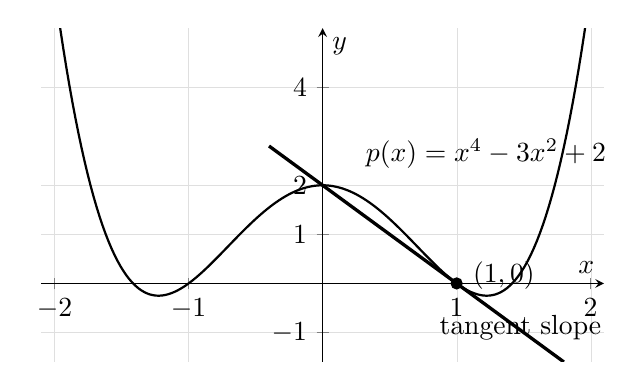
\begin{tikzpicture}
\begin{axis}[
    width=0.72\textwidth,
    height=0.48\textwidth,
    xmin=-2.1, xmax=2.1,
    ymin=-1.6, ymax=5.2,
    axis lines=middle,
    xlabel={\(x\)},
    ylabel={\(y\)},
    xtick={-2,-1,0,1,2},
    ytick={-1,0,1,2,4},
    grid=both,
    grid style={line width=.1pt, draw=gray!25},
]
\addplot[thick, domain=-2:2, samples=180] {x^4-3*x^2+2};
\addplot[very thick, domain=-0.4:1.8, samples=2] {-2*x+2};
\addplot[only marks, mark=*] coordinates {(1,0)};
\node[anchor=west] at (axis cs:1.05,0.15) {\((1,0)\)};
\node[anchor=west] at (axis cs:0.25,2.65) {\(p(x)=x^4-3x^2+2\)};
\node[anchor=west] at (axis cs:0.8,-0.9) {tangent slope \(-2\)};
\end{axis}
\end{tikzpicture}
\caption{The derivative formula gives the tangent slope without returning to the limit definition.}
\label{fig:polynomial-tangent-first-formulas}
\end{figure}

\subsection{Derivative notation in formulas}
\label{subsec:derivative-notation-formulas}

A derivative formula gives a new function.  For example,

\[
\frac{d}{dx}x^3=3x^2
\]

means that the derivative function of

\[
f(x)=x^3
\]

is

\[
f'(x)=3x^2.
\]

At a particular point, we substitute after differentiating.  For instance,

\[
\left.\frac{d}{dx}x^3\right|_{x=2}
=
3(2)^2
=
12.
\]

So

\[
\frac{d}{dx}x^3=3x^2
\]

is a formula for all \(x\), while

\[
\left.\frac{d}{dx}x^3\right|_{x=2}=12
\]

is one slope at one point.

\begin{quote}
\textbf{Differentiate first, then evaluate.}
A formula like

\[
p'(x)=30x^5-6x^2+7
\]

describes slopes along the whole graph.  A number like

\[
p'(1)
\]

is the slope at one point.
\end{quote}

\subsection{What we have proved so far}
\label{subsec:first-derivative-formulas-summary}

The first derivative formulas are:

\[
\boxed{
\frac{d}{dx}(c)=0,
}
\]

\[
\boxed{
\frac{d}{dx}(x)=1,
}
\]

\[
\boxed{
\frac{d}{dx}(x^n)=nx^{n-1}
\qquad(n=1,2,3,\ldots),
}
\]

\[
\boxed{
\frac{d}{dx}\bigl(c f(x)\bigr)=c f'(x),
}
\]

and

\[
\boxed{
\frac{d}{dx}\bigl(f(x)+g(x)\bigr)=f'(x)+g'(x).
}
\]

These rules are enough to differentiate every polynomial.

\paragraph{Example.}
For

\[
q(x)=-4x^5+9x^2-\frac12x+8,
\]

we have

\[
q'(x)
=
-20x^4+18x-\frac12.
\]

Each term is handled separately.  The constant \(8\) contributes nothing to the derivative because it does not affect change.

\subsection{What these formulas do not yet cover}
\label{subsec:first-formulas-do-not-cover}

The rules in this section are useful, but they are not enough for most functions.

They do not yet tell us how to differentiate

\[
x^2\sin x,
\]

or

\[
\frac{x^2+1}{x-3},
\]

or

\[
\sqrt{1+x^2},
\]

or

\[
\sin(x^2).
\]

These functions are built not only by adding and scaling, but also by multiplying, dividing, and putting one function inside another.

The next chapter develops the algebra of derivatives.  The goal is not to memorize more rules for their own sake.  The goal is to make the derivative practical while keeping its meaning: a local rate of change, a tangent slope, and the coefficient of the best linear approximation.
\section{Motion revisited}
\label{sec:motion-revisited}

The derivative began as velocity.  Then it became slope, local linear approximation, and a function of position along a graph.  Now the original motion story returns, but with sharper language.

A position function tells where an object is.  Its derivative tells how fast that position is changing.  The derivative of the derivative tells how fast the velocity is changing.

\subsection{Position, velocity, and acceleration}
\label{subsec:position-velocity-acceleration}

Suppose a cart moves along a straight track.  Its position after \(t\) seconds is

\[
s(t)=t^2
\]

meters, measured from a chosen origin on the track.

At \(t=0\),

\[
s(0)=0.
\]

At \(t=1\),

\[
s(1)=1.
\]

At \(t=2\),

\[
s(2)=4.
\]

The cart is moving farther and farther from the origin, and it is doing so faster as time passes.

The velocity is the derivative of position:

\[
v(t)=s'(t).
\]

Since

\[
s(t)=t^2,
\]

we have

\[
v(t)=2t.
\]

So

\[
v(1)=2\text{ meters/second},
\qquad
v(2)=4\text{ meters/second}.
\]

The velocity itself is changing.  The rate of change of velocity is called acceleration.

Since

\[
v(t)=2t,
\]

we have

\[
a(t)=v'(t)=2.
\]

So the acceleration is constant:

\[
2\text{ meters/second}^2.
\]

\begin{quote}
\textbf{Position, velocity, and acceleration.}
If \(s(t)\) is the position of an object moving along a line, then

\[
\boxed{v(t)=s'(t)}
\]

is its velocity, and

\[
\boxed{a(t)=v'(t)=s''(t)}
\]

is its acceleration.
\end{quote}

The notation

\[
s''(t)
\]

means the derivative of the derivative.  In Leibniz notation,

\[
v(t)=\frac{ds}{dt},
\]

and

\[
a(t)=\frac{dv}{dt}=\frac{d^2s}{dt^2}.
\]

The notation

\[
\frac{d^2s}{dt^2}
\]

means ``differentiate \(s\) twice with respect to \(t\).''  It does not mean

\[
\left(\frac{ds}{dt}\right)^2.
\]

\paragraph{Units.}
If position is measured in meters and time in seconds, then

\[
s(t)\text{ has units of meters,}
\]

\[
v(t)=s'(t)\text{ has units of meters/second,}
\]

and

\[
a(t)=v'(t)\text{ has units of meters/second}^2.
\]

The units explain the meaning.  Acceleration measures how many meters per second of velocity are gained or lost each second.

\[
\begin{array}{c|c|c}
\textbf{quantity} & \textbf{meaning} & \textbf{units} \\ \hline
s(t) & \text{position} & \text{meters} \\[2pt]
v(t)=s'(t) & \text{rate of change of position} & \text{meters/second} \\[2pt]
a(t)=v'(t)=s''(t) & \text{rate of change of velocity} & \text{meters/second}^2
\end{array}
\]

\paragraph{Example.}
Let

\[
s(t)=10+4t-t^2
\]

be the position of a particle in meters after \(t\) seconds.

Then

\[
v(t)=s'(t)=4-2t,
\]

and

\[
a(t)=v'(t)=-2.
\]

At \(t=0\),

\[
v(0)=4,
\]

so the particle is moving in the positive direction.

At \(t=2\),

\[
v(2)=4-4=0.
\]

The particle is momentarily stopped.

At \(t=3\),

\[
v(3)=4-6=-2.
\]

The particle is now moving in the negative direction.

The acceleration is

\[
-2\text{ meters/second}^2
\]

at every time.  This means the velocity is decreasing by \(2\) meters/second each second.

\begin{figure}[h]
\centering
\begin{minipage}{0.32\textwidth}
\centering
\begin{tikzpicture}
\begin{axis}[
    width=\textwidth,
    height=0.82\textwidth,
    xmin=0, xmax=4,
    ymin=8, ymax=15,
    axis lines=left,
    xlabel={\(t\)},
    ylabel={\(s(t)\)},
    xtick={0,2,4},
    ytick={10,14},
    grid=both,
    grid style={line width=.1pt, draw=gray!25},
]
\addplot[thick, domain=0:4, samples=120] {10+4*x-x^2};
\addplot[only marks, mark=*] coordinates {(2,14)};
\node[anchor=south] at (axis cs:2,14.1) {\(v=0\)};
\end{axis}
\end{tikzpicture}
\end{minipage}
\hfill
\begin{minipage}{0.32\textwidth}
\centering
\begin{tikzpicture}
\begin{axis}[
    width=\textwidth,
    height=0.82\textwidth,
    xmin=0, xmax=4,
    ymin=-5, ymax=5,
    axis lines=middle,
    xlabel={\(t\)},
    ylabel={\(v(t)\)},
    xtick={0,2,4},
    ytick={-4,0,4},
    grid=both,
    grid style={line width=.1pt, draw=gray!25},
]
\addplot[very thick, domain=0:4, samples=2] {4-2*x};
\addplot[only marks, mark=*] coordinates {(2,0)};
\end{axis}
\end{tikzpicture}
\end{minipage}
\hfill
\begin{minipage}{0.32\textwidth}
\centering
\begin{tikzpicture}
\begin{axis}[
    width=\textwidth,
    height=0.82\textwidth,
    xmin=0, xmax=4,
    ymin=-4, ymax=2,
    axis lines=middle,
    xlabel={\(t\)},
    ylabel={\(a(t)\)},
    xtick={0,2,4},
    ytick={-2,0},
    grid=both,
    grid style={line width=.1pt, draw=gray!25},
]
\addplot[very thick, domain=0:4, samples=2] {-2};
\node[anchor=west] at (axis cs:0.5,-2.35) {\(a(t)=-2\)};
\end{axis}
\end{tikzpicture}
\end{minipage}
\caption{Position, velocity, and acceleration are linked by derivatives.  The position has a maximum when the velocity changes sign from positive to negative.}
\label{fig:position-velocity-acceleration}
\end{figure}

The point \(t=2\) is special.  The position graph has a horizontal tangent there.  The velocity is zero there.  The particle changes direction there.

This is the motion version of a graph idea:

\[
\text{a horizontal tangent means derivative }0.
\]

\subsection{Speed versus velocity}
\label{subsec:speed-versus-velocity}

Velocity has a sign.  Speed does not.

If the positive direction is to the right, then

\[
v(t)>0
\]

means the object is moving right, while

\[
v(t)<0
\]

means the object is moving left.

Speed asks only how fast the object is moving, not which direction it is moving.  For motion along a line,

\[
\boxed{\text{speed}=|v(t)|.}
\]

\paragraph{Example.}
Let

\[
s(t)=t^2-4t,
\qquad 0\le t\le4.
\]

Then

\[
v(t)=s'(t)=2t-4.
\]

At \(t=1\),

\[
v(1)=-2,
\]

so the particle is moving in the negative direction with speed

\[
|v(1)|=2.
\]

At \(t=3\),

\[
v(3)=2,
\]

so the particle is moving in the positive direction with speed

\[
|v(3)|=2.
\]

The velocities are different:

\[
-2
\qquad\text{and}\qquad
2,
\]

but the speeds are the same:

\[
2
\qquad\text{and}\qquad
2.
\]

At \(t=2\),

\[
v(2)=0.
\]

The particle turns around.

The position values are

\[
s(0)=0,
\qquad
s(2)=-4,
\qquad
s(4)=0.
\]

So from \(t=0\) to \(t=4\), the displacement is

\[
s(4)-s(0)=0.
\]

The average velocity is therefore

\[
\frac{s(4)-s(0)}{4-0}=0.
\]

But the particle did not stand still.  It moved from \(0\) to \(-4\), and then back from \(-4\) to \(0\).  The total distance traveled is

\[
4+4=8.
\]

So the average speed over the interval is

\[
\frac{8}{4}=2.
\]

\[
\boxed{
\text{average velocity}
=
\frac{\text{displacement}}{\text{time}},
\qquad
\text{average speed}
=
\frac{\text{distance traveled}}{\text{time}}.
}
\]

These are not the same when the object changes direction.

\begin{figure}[h]
\centering
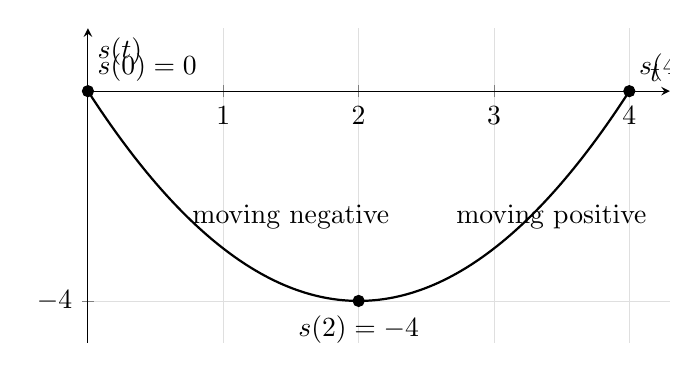
\begin{tikzpicture}
\begin{axis}[
    width=0.74\textwidth,
    height=0.46\textwidth,
    xmin=0, xmax=4.3,
    ymin=-4.8, ymax=1.2,
    axis lines=middle,
    xlabel={\(t\)},
    ylabel={\(s(t)\)},
    xtick={0,1,2,3,4},
    ytick={-4,0},
    grid=both,
    grid style={line width=.1pt, draw=gray!25},
]
\addplot[thick, domain=0:4, samples=120] {x^2-4*x};
\addplot[only marks, mark=*] coordinates {(0,0) (2,-4) (4,0)};
\node[anchor=south west] at (axis cs:0,0) {\(s(0)=0\)};
\node[anchor=north] at (axis cs:2,-4.1) {\(s(2)=-4\)};
\node[anchor=south west] at (axis cs:4,0) {\(s(4)=0\)};
\node[anchor=west] at (axis cs:0.7,-2.4) {moving negative};
\node[anchor=west] at (axis cs:2.65,-2.4) {moving positive};
\end{axis}
\end{tikzpicture}
\caption{The particle returns to its starting position, so its displacement is \(0\), but it has traveled a total distance of \(8\).}
\label{fig:speed-vs-velocity-return}
\end{figure}

There is a small warning hidden here.  Since speed is

\[
|v(t)|,
\]

the speed graph can have a corner when \(v(t)\) passes through \(0\).  In this example,

\[
\text{speed}=|2t-4|.
\]

It has a sharp corner at \(t=2\).  The velocity is a smooth line, but the speed is not smooth at the turning instant.

\subsection{Falling under constant acceleration}
\label{subsec:falling-under-constant-acceleration}

Near the surface of the earth, if air resistance is ignored, falling objects have nearly constant acceleration.

If we measure height upward, then gravity pulls in the negative direction.  In feet, the acceleration is approximately

\[
-32\text{ ft/s}^2.
\]

In meters, it is approximately

\[
-9.8\text{ m/s}^2.
\]

The sign is not a property of gravity alone.  It also depends on our choice of positive direction.  If upward is positive, gravity is negative.  If downward is positive, gravity is positive.

\paragraph{The standard height model in feet.}
Suppose height is measured in feet and time in seconds.  If upward is positive and acceleration is

\[
-32\text{ ft/s}^2,
\]

then a useful height model is

\[
y(t)=y_0+v_0t-16t^2.
\]

Here:

\[
y_0=\text{initial height},
\]

and

\[
v_0=\text{initial velocity}.
\]

Differentiate:

\[
v(t)=y'(t)=v_0-32t.
\]

Differentiate again:

\[
a(t)=v'(t)=-32.
\]

So the formula has exactly the desired acceleration.

In meters, the corresponding model is

\[
y(t)=y_0+v_0t-4.9t^2,
\]

with

\[
v(t)=v_0-9.8t
\]

and

\[
a(t)=-9.8.
\]

\begin{quote}
\textbf{Constant acceleration model.}
If acceleration is constant and equal to \(a\), then

\[
\boxed{s(t)=s_0+v_0t+\frac12at^2}
\]

has

\[
\boxed{v(t)=s'(t)=v_0+at}
\]

and

\[
\boxed{a(t)=s''(t)=a.}
\]

At this point we can verify the formula by differentiating.  Later, integration will explain how to build it from the acceleration.
\end{quote}

\paragraph{Example: a ball thrown upward.}
A ball is thrown upward from the ground with initial velocity

\[
64\text{ ft/s}.
\]

Ignoring air resistance, its height is

\[
y(t)=64t-16t^2.
\]

The velocity is

\[
v(t)=y'(t)=64-32t.
\]

The acceleration is

\[
a(t)=v'(t)=-32.
\]

The ball reaches its highest point when its velocity is \(0\):

\[
64-32t=0.
\]

Thus

\[
t=2.
\]

At that time the height is

\[
y(2)=64(2)-16(2)^2=128-64=64.
\]

So the maximum height is

\[
64\text{ ft}.
\]

The ball returns to the ground when

\[
y(t)=0.
\]

Solve:

\[
64t-16t^2=0.
\]

Factor:

\[
16t(4-t)=0.
\]

Thus

\[
t=0
\qquad\text{or}\qquad
t=4.
\]

The time \(t=0\) is the launch time.  The ball lands at

\[
t=4\text{ seconds}.
\]

At landing,

\[
v(4)=64-32(4)=-64.
\]

So the velocity is

\[
-64\text{ ft/s}.
\]

The speed is

\[
64\text{ ft/s}.
\]

The negative sign says the ball is moving downward.

\begin{figure}[h]
\centering
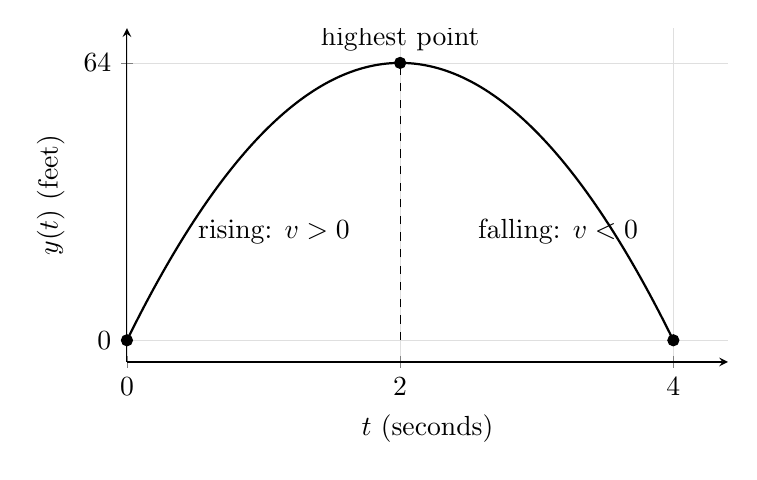
\begin{tikzpicture}
\begin{axis}[
    width=0.76\textwidth,
    height=0.48\textwidth,
    xmin=0, xmax=4.4,
    ymin=-5, ymax=72,
    axis lines=left,
    xlabel={\(t\) (seconds)},
    ylabel={\(y(t)\) (feet)},
    xtick={0,2,4},
    ytick={0,64},
    grid=both,
    grid style={line width=.1pt, draw=gray!25},
]
\addplot[thick, domain=0:4, samples=140] {64*x-16*x^2};
\addplot[only marks, mark=*] coordinates {(0,0) (2,64) (4,0)};
\draw[dashed] (axis cs:2,0) -- (axis cs:2,64);
\node[anchor=south] at (axis cs:2,64.5) {highest point};
\node[anchor=west] at (axis cs:0.45,25) {rising: \(v>0\)};
\node[anchor=west] at (axis cs:2.5,25) {falling: \(v<0\)};
\end{axis}
\end{tikzpicture}
\caption{At the highest point, the velocity is \(0\), but the acceleration is still \(-32\text{ ft/s}^2\).}
\label{fig:thrown-upward}
\end{figure}

This example corrects a common misunderstanding:

\[
\boxed{
\text{At the top, velocity is }0,\text{ but acceleration is not }0.
}
\]

Gravity does not turn off at the highest point.  The velocity is momentarily zero, but it is still changing.

\subsection{Units and signs in motion problems}
\label{subsec:units-signs-motion}

The hardest part of many motion problems is not differentiating.  It is deciding what the signs mean.

A position is measured relative to an origin.  A velocity is measured relative to a positive direction.  Acceleration tells whether velocity is increasing or decreasing in that chosen direction.

\[
\begin{array}{c|l}
\textbf{statement} & \textbf{meaning} \\ \hline
s(t)>0 & \text{the object is on the positive side of the origin} \\[2pt]
s(t)<0 & \text{the object is on the negative side of the origin} \\[2pt]
v(t)>0 & \text{the object is moving in the positive direction} \\[2pt]
v(t)<0 & \text{the object is moving in the negative direction} \\[2pt]
a(t)>0 & \text{the velocity is increasing} \\[2pt]
a(t)<0 & \text{the velocity is decreasing}
\end{array}
\]

Acceleration does not directly tell which way the object is moving.  Velocity does that.

Acceleration tells how velocity is changing.

\paragraph{Speeding up and slowing down.}
Because speed is

\[
|v(t)|,
\]

an object speeds up when the magnitude of velocity increases.

For motion along a line:

\[
\boxed{
\text{if \(v\) and \(a\) have the same sign, the object is speeding up,}
}
\]

and

\[
\boxed{
\text{if \(v\) and \(a\) have opposite signs, the object is slowing down.}
}
\]

\[
\begin{array}{c|c|c}
\textbf{velocity} & \textbf{acceleration} & \textbf{speed} \\ \hline
v>0 & a>0 & \text{increasing} \\[2pt]
v>0 & a<0 & \text{decreasing} \\[2pt]
v<0 & a>0 & \text{decreasing} \\[2pt]
v<0 & a<0 & \text{increasing}
\end{array}
\]

For the ball

\[
y(t)=64t-16t^2,
\]

we have

\[
v(t)=64-32t,
\qquad
a(t)=-32.
\]

For \(0<t<2\),

\[
v(t)>0
\]

and

\[
a(t)<0.
\]

The signs are opposite, so the ball is slowing down as it rises.

For \(2<t<4\),

\[
v(t)<0
\]

and

\[
a(t)<0.
\]

The signs are the same, so the ball is speeding up as it falls.

\paragraph{Same physical motion, different sign convention.}
Suppose a stone is dropped from a \(100\)-meter tower.

If height above the ground is the position, and upward is positive, then

\[
y(t)=100-4.9t^2.
\]

The velocity is

\[
v(t)=-9.8t,
\]

and the acceleration is

\[
a(t)=-9.8.
\]

Both velocity and acceleration are negative after the stone is released, so the stone is speeding up downward.

If instead we measure downward distance from the release point, then the same motion is described by

\[
r(t)=4.9t^2.
\]

Then

\[
r'(t)=9.8t,
\]

and

\[
r''(t)=9.8.
\]

Now velocity and acceleration are positive because the positive direction has been chosen downward.

The physics did not change.  The coordinate choice changed.

\begin{quote}
\textbf{Sign rule for motion.}
Before interpreting signs, choose:

\[
\text{origin}
\qquad\text{and}\qquad
\text{positive direction}.
\]

Only then do signs have meaning.
\end{quote}

\paragraph{A small checklist for motion problems.}
For a motion problem on a line:

\[
\begin{array}{ll}
1. & \text{Choose an origin and a positive direction.}\\
2. & \text{Write the position function with units.}\\
3. & \text{Differentiate once for velocity.}\\
4. & \text{Differentiate twice for acceleration.}\\
5. & \text{Use \(|v(t)|\) when the question asks for speed.}
\end{array}
\]

The derivative has now returned to its first meaning: instantaneous motion.  But even motion can hide traps.  A graph may look continuous and still have no velocity at a sharp turn.  A derivative may exist and still behave unexpectedly.  Before moving to a larger library of differentiation rules, we pause to collect these warning examples.
\section{Warning examples}
\label{sec:derivative-warning-examples}

Motion gives the derivative a natural meaning.  It also shows why the derivative is a demanding idea.  A position can be continuous and still have no velocity at one instant.  A derivative can exist and still behave badly nearby.  A graph can look harmless because the picture has missed the trouble.

These examples are not exceptions to the theory.  They are the reason the definitions were made carefully.

\subsection{A continuous function with no derivative at one point}
\label{subsec:continuous-no-derivative-one-point}

Imagine a particle moving along a line with position

\[
s(t)=|t|.
\]

At \(t=-2\),

\[
s(-2)=2.
\]

At \(t=-1\),

\[
s(-1)=1.
\]

At \(t=0\),

\[
s(0)=0.
\]

Then after \(t=0\), the particle moves away again:

\[
s(1)=1,
\qquad
s(2)=2.
\]

The position is continuous.  The particle does not teleport.  But at \(t=0\), it reverses direction instantly.

The derivative at \(0\), if it existed, would be

\[
s'(0)
=
\lim_{h\to0}\frac{s(0+h)-s(0)}{h}
=
\lim_{h\to0}\frac{|h|}{h}.
\]

For \(h>0\),

\[
\frac{|h|}{h}=1.
\]

For \(h<0\),

\[
\frac{|h|}{h}=-1.
\]

So the right-hand limiting slope is

\[
1,
\]

while the left-hand limiting slope is

\[
-1.
\]

There is no single limiting slope.  Therefore

\[
s'(0)
\]

does not exist.

\begin{figure}[h]
\centering
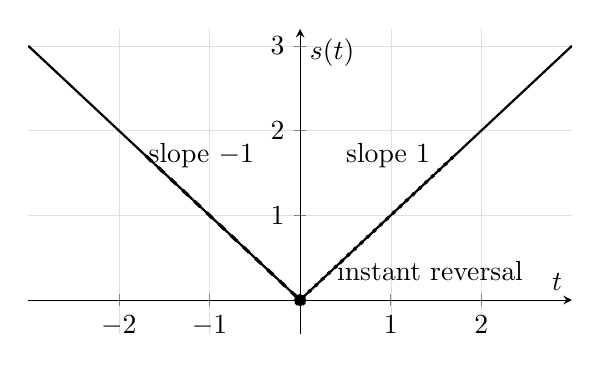
\begin{tikzpicture}
\begin{axis}[
    width=0.70\textwidth,
    height=0.45\textwidth,
    xmin=-3, xmax=3,
    ymin=-0.4, ymax=3.2,
    axis lines=middle,
    xlabel={\(t\)},
    ylabel={\(s(t)\)},
    xtick={-2,-1,0,1,2},
    ytick={1,2,3},
    grid=both,
    grid style={line width=.1pt, draw=gray!25},
]
\addplot[thick, domain=-3:0, samples=2] {-x};
\addplot[thick, domain=0:3, samples=2] {x};
\addplot[only marks, mark=*] coordinates {(0,0)};
\addplot[very thick, dashed, domain=-1.7:0.05, samples=2] {-x};
\addplot[very thick, dotted, domain=-0.05:1.7, samples=2] {x};
\node[anchor=east] at (axis cs:-0.4,1.7) {slope \(-1\)};
\node[anchor=west] at (axis cs:0.4,1.7) {slope \(1\)};
\node[anchor=west] at (axis cs:0.3,0.35) {instant reversal};
\end{axis}
\end{tikzpicture}
\caption{The function \(s(t)=|t|\) is continuous at \(0\), but it has no derivative there.}
\label{fig:absolute-value-motion-warning}
\end{figure}

This example is the motion version of a corner.  The particle has a position at every nearby time.  The position changes without a break.  But the direction of motion changes too abruptly for there to be one instantaneous velocity at \(t=0\).

\begin{quote}
\textbf{Continuity is not enough.}
Continuity controls nearby values:

\[
s(t)\to s(0).
\]

Differentiability controls nearby slopes:

\[
\frac{s(0+h)-s(0)}{h}.
\]

The second condition is stronger.
\end{quote}

There is a useful way to say the same thing with local linear approximation.  If \(s\) were differentiable at \(0\), then near \(0\) we would have

\[
|h| \approx mh
\]

for one fixed slope \(m\).  But for \(h>0\), this would require \(m=1\), while for \(h<0\), it would require \(m=-1\).  One line cannot model both sides to first order.

The graph is unbroken, but it is not locally linear at the corner.

\subsection{Optional: a derivative that exists but is not continuous}
\label{subsec:derivative-exists-not-continuous}

A first mental picture might say:

\[
\text{if a derivative exists, then it should vary smoothly.}
\]

That picture is too optimistic.  A function can be differentiable at a point even though its derivative is not continuous there.

The example is a little more advanced because it uses a sine function inside a rapidly oscillating expression.  The only new idea is that oscillation can be hidden by a small factor.

Define

\[
f(x)=
\begin{cases}
x^2\sin\left(\dfrac1x\right), & x\neq0,\\[8pt]
0, & x=0.
\end{cases}
\]

First, \(f\) is continuous at \(0\).  Since

\[
-1\le \sin\left(\frac1x\right)\le 1,
\]

we have

\[
-x^2\le x^2\sin\left(\frac1x\right)\le x^2.
\]

As \(x\to0\), both \(-x^2\) and \(x^2\) approach \(0\).  So by squeezing,

\[
\lim_{x\to0}x^2\sin\left(\frac1x\right)=0=f(0).
\]

Now compute the derivative at \(0\) from the definition:

\[
f'(0)
=
\lim_{h\to0}\frac{f(h)-f(0)}{h}.
\]

For \(h\neq0\),

\[
\frac{f(h)-f(0)}{h}
=
\frac{h^2\sin\left(\frac1h\right)}{h}
=
h\sin\left(\frac1h\right).
\]

Again,

\[
\left|h\sin\left(\frac1h\right)\right|\le |h|.
\]

Therefore

\[
\lim_{h\to0}h\sin\left(\frac1h\right)=0.
\]

So

\[
\boxed{f'(0)=0.}
\]

The derivative exists at \(0\).

But the derivative function is not continuous at \(0\).  Using derivative rules that will be proved in the next chapter, for \(x\neq0\) one finds

\[
f'(x)
=
2x\sin\left(\frac1x\right)
-
\cos\left(\frac1x\right).
\]

The first term approaches \(0\), but the second term oscillates.

To see this clearly, take

\[
x_n=\frac{1}{2\pi n}.
\]

Then \(x_n\to0\), and

\[
\cos\left(\frac1{x_n}\right)
=
\cos(2\pi n)
=
1.
\]

Also,

\[
\sin\left(\frac1{x_n}\right)
=
\sin(2\pi n)
=
0.
\]

So

\[
f'(x_n)=-1.
\]

Now take

\[
y_n=\frac{1}{(2n+1)\pi}.
\]

Then \(y_n\to0\), and

\[
\cos\left(\frac1{y_n}\right)
=
\cos((2n+1)\pi)
=
-1.
\]

Also,

\[
\sin\left(\frac1{y_n}\right)=0.
\]

So

\[
f'(y_n)=1.
\]

Thus as \(x\to0\), the derivative values get arbitrarily close to both \(-1\) and \(1\) along different sequences.  Therefore

\[
\lim_{x\to0}f'(x)
\]

does not exist.

But

\[
f'(0)=0.
\]

So \(f'\) is not continuous at \(0\).

\begin{quote}
\textbf{Differentiable does not mean continuously differentiable.}
A function may have a derivative at a point even though the derivative function behaves badly near that point.
\end{quote}

This example separates two properties:

\[
\text{\(f\) is differentiable}
\]

and

\[
\text{\(f'\) is continuous.}
\]

The second property is stronger.  Many functions in applications have continuous derivatives, and they are pleasant to work with.  But the definition of derivative does not promise continuity of \(f'\).

\subsection{A graphing calculator can miss a sharp corner}
\label{subsec:calculator-misses-corner}

Graphs are useful, but a graph on a screen is not the function.  A screen shows finitely many pixels.  A calculator or computer often samples finitely many points and connects them.  If the important feature lies between sampled points, the picture may miss it.

Consider

\[
K(x)=|x-0.03|.
\]

This graph has a sharp corner at

\[
x=0.03.
\]

At that point,

\[
K(0.03)=0.
\]

The derivative does not exist there, because the left-hand slope is \(-1\) and the right-hand slope is \(1\).

Indeed, for \(h<0\),

\[
\frac{K(0.03+h)-K(0.03)}{h}
=
\frac{|h|}{h}
=
-1,
\]

while for \(h>0\),

\[
\frac{K(0.03+h)-K(0.03)}{h}
=
\frac{|h|}{h}
=
1.
\]

But suppose a graphing program samples only at

\[
x=-0.4,-0.3,-0.2,-0.1,0,0.1,0.2,0.3,0.4.
\]

Then it never samples the corner at \(x=0.03\).  The plotted points near the corner are

\[
(0,0.03)
\qquad\text{and}\qquad
(0.1,0.07).
\]

Connecting those two points draws a line segment that hides the actual sharp turn.

\begin{figure}[h]
\centering
\begin{minipage}{0.48\textwidth}
\centering
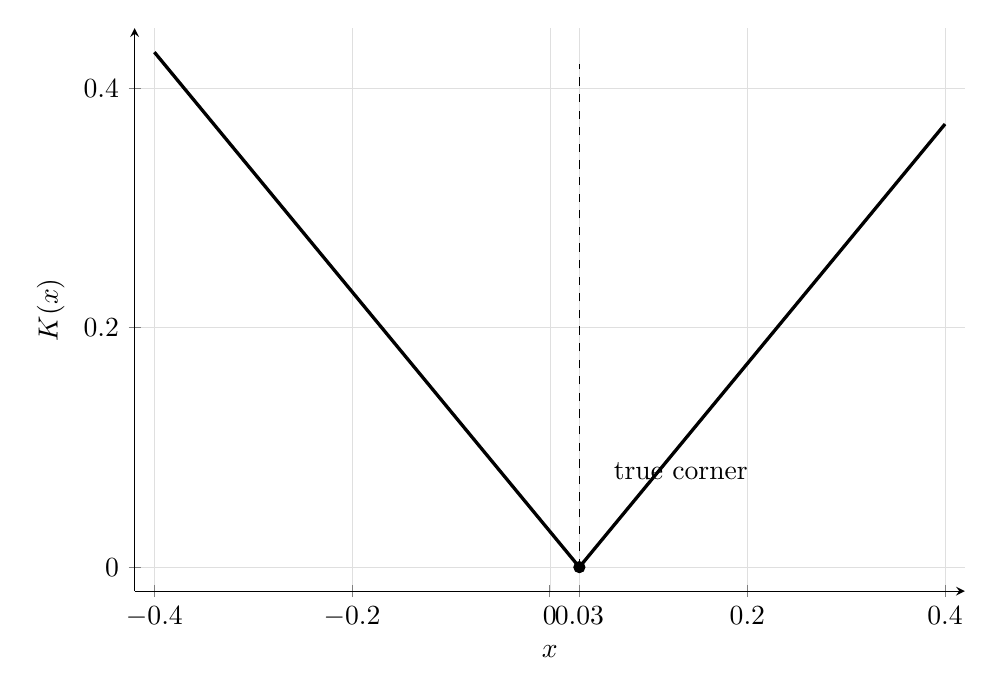
\begin{tikzpicture}
\begin{axis}[
    width=\textwidth,
    height=0.72\textwidth,
    xmin=-0.42, xmax=0.42,
    ymin=-0.02, ymax=0.45,
    axis lines=left,
    xlabel={\(x\)},
    ylabel={\(K(x)\)},
    xtick={-0.4,-0.2,0,0.03,0.2,0.4},
    xticklabels={\(-0.4\),\(-0.2\),\(0\),\(0.03\),\(0.2\),\(0.4\)},
    ytick={0,0.2,0.4},
    grid=both,
    grid style={line width=.1pt, draw=gray!25},
]
\addplot[very thick, domain=-0.4:0.03, samples=2] {0.03-x};
\addplot[very thick, domain=0.03:0.4, samples=2] {x-0.03};
\addplot[only marks, mark=*] coordinates {(0.03,0)};
\draw[dashed] (axis cs:0.03,0) -- (axis cs:0.03,0.42);
\node[anchor=west] at (axis cs:0.055,0.08) {true corner};
\end{axis}
\end{tikzpicture}

\smallskip
\(\text{The actual graph}\)
\end{minipage}
\hfill
\begin{minipage}{0.48\textwidth}
\centering
\begin{tikzpicture}
\begin{axis}[
    width=\textwidth,
    height=0.72\textwidth,
    xmin=-0.42, xmax=0.42,
    ymin=-0.02, ymax=0.45,
    axis lines=left,
    xlabel={\(x\)},
    ylabel={\(K(x)\)},
    xtick={-0.4,-0.2,0,0.2,0.4},
    ytick={0,0.2,0.4},
    grid=both,
    grid style={line width=.1pt, draw=gray!25},
]
\addplot[thick, dashed, mark=*] coordinates {
    (-0.4,0.43)
    (-0.3,0.33)
    (-0.2,0.23)
    (-0.1,0.13)
    (0,0.03)
    (0.1,0.07)
    (0.2,0.17)
    (0.3,0.27)
    (0.4,0.37)
};
\node[anchor=west] at (axis cs:0.02,0.16) {corner missed};
\end{axis}
\end{tikzpicture}

\smallskip
\(\text{A coarse sampled plot}\)
\end{minipage}
\caption{A finite plot can miss a nondifferentiable point if it is not sampled.}
\label{fig:calculator-misses-corner}
\end{figure}

The lesson is not that calculators are bad.  The lesson is that a picture is evidence, not proof.  A graph can suggest where to look.  The derivative definition decides what is true.

\begin{quote}
\textbf{Safe test for differentiability.}
To know whether \(f'(a)\) exists, examine

\[
\lim_{h\to0}\frac{f(a+h)-f(a)}{h}.
\]

A graph may guide the eye, but the difference quotient tests the point.
\end{quote}

The warnings in this section protect the meaning of the derivative.

\[
\begin{array}{c|c}
\textbf{what can happen} & \textbf{what it teaches} \\ \hline
\text{continuous but not differentiable} & \text{nearby values are not enough} \\[2pt]
\text{derivative exists but is not continuous} & \text{a derivative can behave irregularly} \\[2pt]
\text{calculator misses a corner} & \text{finite sampling is not proof}
\end{array}
\]

The derivative is now defined, interpreted, and tested.  But computing every derivative from the limit definition is too slow.  The next chapter builds a faster language: rules for differentiating sums, products, quotients, compositions, and the elementary functions.
\section{Chapter review and discovery problems}
\label{sec:chapter-review-derivative}

The chapter began with a familiar quotient:

\[
\frac{f(b)-f(a)}{b-a}.
\]

That quotient measured average change.  By shrinking the interval, we found a new number:

\[
f'(a)=\lim_{h\to0}\frac{f(a+h)-f(a)}{h}.
\]

The same number appeared in several forms.  It was an instantaneous rate, a tangent slope, the coefficient in the best linear approximation, and velocity when the function was position.

\[
\begin{array}{c|c}
\textbf{idea} & \textbf{formula} \\ \hline
\text{average rate of change} &
\dfrac{f(b)-f(a)}{b-a} \\[10pt]
\text{derivative at }a &
f'(a)=\displaystyle\lim_{h\to0}\dfrac{f(a+h)-f(a)}{h} \\[12pt]
\text{tangent line at }a &
y-f(a)=f'(a)(x-a) \\[8pt]
\text{local linear approximation} &
f(a+h)\approx f(a)+f'(a)h \\[8pt]
\text{differential approximation} &
dy=f'(x)\,dx \\[8pt]
\text{motion} &
v(t)=s'(t),\qquad a(t)=v'(t)=s''(t)
\end{array}
\]

\begin{figure}[h]
\centering
\begin{tikzpicture}[every node/.style={font=\small}]
  \node[draw, rounded corners, align=center, minimum width=3.2cm, minimum height=0.85cm] (avg) at (0,0)
  {average rate\\ \(\dfrac{f(b)-f(a)}{b-a}\)};

  \node[draw, rounded corners, align=center, minimum width=3.2cm, minimum height=0.85cm] (lim) at (5,0)
  {limit of rates\\ \(f'(a)\)};

  \node[draw, rounded corners, align=center, minimum width=3.2cm, minimum height=0.85cm] (tan) at (0,-2.0)
  {tangent slope\\ at one point};

  \node[draw, rounded corners, align=center, minimum width=3.2cm, minimum height=0.85cm] (lin) at (5,-2.0)
  {local line\\ \(f(a+h)\approx f(a)+f'(a)h\)};

  \node[draw, rounded corners, align=center, minimum width=3.2cm, minimum height=0.85cm] (motion) at (2.5,-4.0)
  {motion\\ \(v=s'\), \(a=v'\)};

  \draw[->, thick] (avg) -- (lim);
  \draw[->, thick] (lim) -- (tan);
  \draw[->, thick] (tan) -- (lin);
  \draw[->, thick] (lin) -- (motion);
  \draw[->, thick] (motion) -- (avg);
\end{tikzpicture}
\caption{The derivative is one idea with several connected meanings.}
\label{fig:chapter4-derivative-map}
\end{figure}

The problems below are meant to make those meanings fluent.  Some ask for calculations.  Some ask for explanations.  Some ask for judgment.  Calculus needs all three.

\subsection{Skills: derivative from definition}
\label{subsec:skills-derivative-from-definition}

Use the definition

\[
f'(a)=\lim_{h\to0}\frac{f(a+h)-f(a)}{h}
\]

unless the problem explicitly says otherwise.  Show the algebra that removes the factor \(h\) before taking the limit.

\paragraph{Derivatives at a point.}
Find \(f'(a)\).

\begin{enumerate}
\item
\[
f(x)=x^2,\qquad a=-1.
\]

\item
\[
f(x)=x^2,\qquad a=5.
\]

\item
\[
f(x)=x^3,\qquad a=1.
\]

\item
\[
f(x)=x^3,\qquad a=-2.
\]

\item
\[
f(x)=5x-7,\qquad a=4.
\]

\item
\[
f(x)=3x^2-2x+1,\qquad a=2.
\]

\item
\[
f(x)=\frac1x,\qquad a=2.
\]

\item
\[
f(x)=\frac1{x+1},\qquad a=0.
\]

\item
\[
f(x)=\sqrt{x},\qquad a=9.
\]

\item
\[
f(x)=\sqrt{x},\qquad a=4.
\]
\end{enumerate}

\paragraph{Derivative functions.}
Use the definition to find \(f'(x)\).  State where your formula is valid.

\begin{enumerate}
\setcounter{enumi}{10}

\item
\[
f(x)=x^2+3x.
\]

\item
\[
f(x)=x^3-4x.
\]

\item
\[
f(x)=2x^2-5x+8.
\]

\item
\[
f(x)=\frac1x.
\]

\item
\[
f(x)=\sqrt{x}.
\]

\item
\[
f(x)=\frac{1}{x-2}.
\]
\end{enumerate}

\paragraph{Using the first derivative formulas.}
Differentiate.

\begin{enumerate}
\setcounter{enumi}{16}

\item
\[
p(x)=4x^5-3x^2+7x-9.
\]

\item
\[
q(x)=-2x^6+5x^3-\frac12x+10.
\]

\item
\[
r(x)=x^4-4x^3+6x^2-4x+1.
\]

\item
\[
s(x)=7.
\]

\item
\[
m(x)=3x^2+2x+1.
\]

Find

\[
m'(0),\qquad m'(1),\qquad m'(-1).
\]

\item
\[
P(x)=x^4-2x^2.
\]

Find all \(x\)-values where the tangent line is horizontal.
\end{enumerate}

\paragraph{Tangent lines.}
Find the equation of the tangent line at the given point.

\begin{enumerate}
\setcounter{enumi}{22}

\item
\[
f(x)=x^2,\qquad x=3.
\]

\item
\[
f(x)=x^3,\qquad x=2.
\]

\item
\[
f(x)=3x^2-5x+1,\qquad x=1.
\]

\item
\[
f(x)=\frac1x,\qquad x=1.
\]

\item
\[
f(x)=\sqrt{x},\qquad x=4.
\]

\item
For

\[
p(x)=x^4-3x^2+2,
\]

find the tangent line at \(x=-1\).
\end{enumerate}

\paragraph{Local linear approximation.}
Use

\[
f(a+h)\approx f(a)+f'(a)h.
\]

\begin{enumerate}
\setcounter{enumi}{28}

\item Use \(f(x)=x^2\) at \(a=5\) to estimate

\[
(5.03)^2.
\]

Then compute the exact value and the error.

\item Use \(f(x)=\sqrt{x}\) at \(a=9\) to estimate

\[
\sqrt{9.2}.
\]

\item Use \(f(x)=1/x\) at \(a=2\) to estimate

\[
\frac1{2.01}.
\]

\item Let

\[
f(x)=x^3.
\]

Use the linearization at \(a=2\) to estimate

\[
(2.02)^3.
\]

Then compare with the exact value.

\item Let

\[
A(r)=\pi r^2.
\]

Use differentials to estimate the change in area when the radius changes from \(10\) cm to \(10.1\) cm.

\item Let

\[
V(x)=x^3.
\]

Use differentials to estimate the change in volume of a cube when the side length changes from \(4\) cm to \(4.05\) cm.
\end{enumerate}

\paragraph{Differentiability and continuity.}
Decide whether the derivative exists at the indicated point.  Explain using the difference quotient or one-sided slopes.

\begin{enumerate}
\setcounter{enumi}{34}

\item
\[
f(x)=|x|,\qquad a=0.
\]

\item
\[
f(x)=|x-3|,\qquad a=3.
\]

\item
\[
f(x)=
\begin{cases}
x, & x<1,\\
2x-1, & x\ge1,
\end{cases}
\qquad a=1.
\]

\item
\[
f(x)=
\begin{cases}
x^2, & x<0,\\
x, & x\ge0,
\end{cases}
\qquad a=0.
\]

\item
\[
f(x)=\sqrt[3]{x},\qquad a=0.
\]

\item
\[
f(x)=|x|^{2/3},\qquad a=0.
\]
\end{enumerate}

\paragraph{Motion.}
Let \(s(t)\) be position in meters after \(t\) seconds.

\begin{enumerate}
\setcounter{enumi}{40}

\item If

\[
s(t)=t^2+3t,
\]

find \(v(t)\) and \(a(t)\).  Find the velocity and acceleration at \(t=2\).

\item If

\[
s(t)=10+6t-t^2,
\]

find the time when the object is momentarily stopped.

\item If

\[
s(t)=t^2-4t,
\qquad 0\le t\le4,
\]

find the displacement, total distance traveled, average velocity, and average speed on the interval \([0,4]\).

\item A ball is thrown upward with height

\[
y(t)=80t-16t^2
\]

feet after \(t\) seconds.  Find the velocity, acceleration, time of maximum height, maximum height, and time when the ball returns to the ground.

\item A stone is dropped from a height of \(144\) feet.  Its height is

\[
y(t)=144-16t^2.
\]

Find its velocity at impact.

\item Suppose

\[
s(t)=t^3-6t^2+9t.
\]

Find \(v(t)\).  Determine when the particle is moving in the positive direction and when it is moving in the negative direction.
\end{enumerate}

\subsection{Concept check: tangent line versus secant line}
\label{subsec:concept-check-tangent-secant}

Answer in complete sentences where appropriate.

\begin{enumerate}
\item What is the difference between a secant line and a tangent line?

\item Why does the difference quotient

\[
\frac{f(a+h)-f(a)}{h}
\]

require \(h\neq0\)?

\item Why can the limit of the difference quotient still exist even though the quotient itself is not defined at \(h=0\)?

\item A tangent line is sometimes described as a line that ``just touches'' a curve.  Why is this description unreliable?

\item Give an example of a tangent line that crosses the curve at the point of tangency.

\item What does the statement

\[
f'(3)=7
\]

mean geometrically?

\item What does the statement

\[
s'(3)=7
\]

mean if \(s(t)\) is measured in meters and \(t\) is measured in seconds?

\item Suppose

\[
f'(a)=0.
\]

Must \(f\) have a local maximum or local minimum at \(a\)?  Give an example.

\item Suppose \(f\) is differentiable at \(a\).  What must be true about \(f\) at \(a\)?

\item Suppose \(f\) is continuous at \(a\).  Must \(f\) be differentiable at \(a\)?  Give an example.

\item Why is the derivative best understood as a local idea?

\item Explain the meaning of

\[
f(a+h)=f(a)+f'(a)h+E(h),
\qquad
\frac{E(h)}{h}\to0.
\]

\item What is the difference between \(\Delta y\) and \(dy\)?

\item In the approximation

\[
\Delta y\approx dy=f'(x)\,dx,
\]

which quantity is exact and which quantity is linearized?

\item If \(f'(a)\) is large in magnitude, what does that say about the sensitivity of \(f\) near \(a\)?

\item In one-dimensional motion, why is speed equal to \(|v(t)|\) rather than \(v(t)\)?

\item Can an object have velocity \(0\) and nonzero acceleration at the same instant?  Give an example.

\item A particle has \(v(t)<0\) and \(a(t)<0\).  Is it speeding up or slowing down?  Explain.

\item A particle has \(v(t)>0\) and \(a(t)<0\).  Is it speeding up or slowing down?  Explain.

\item Why can a graphing calculator miss a nondifferentiable point?
\end{enumerate}

\subsection{Project: estimating velocity from noisy position data}
\label{subsec:project-noisy-position-data}

A motion sensor records position once every half-second.  The object moves along a straight track.  The sensor is good, but not perfect.  Its readings contain small measurement errors.

\[
\begin{array}{c|ccccccccc}
t\text{ (seconds)} & 0 & 0.5 & 1.0 & 1.5 & 2.0 & 2.5 & 3.0 & 3.5 & 4.0 \\ \hline
s(t)\text{ (meters)} & 0.03 & 1.18 & 3.08 & 5.17 & 8.04 & 11.19 & 15.06 & 19.18 & 24.05
\end{array}
\]

\begin{figure}[h]
\centering
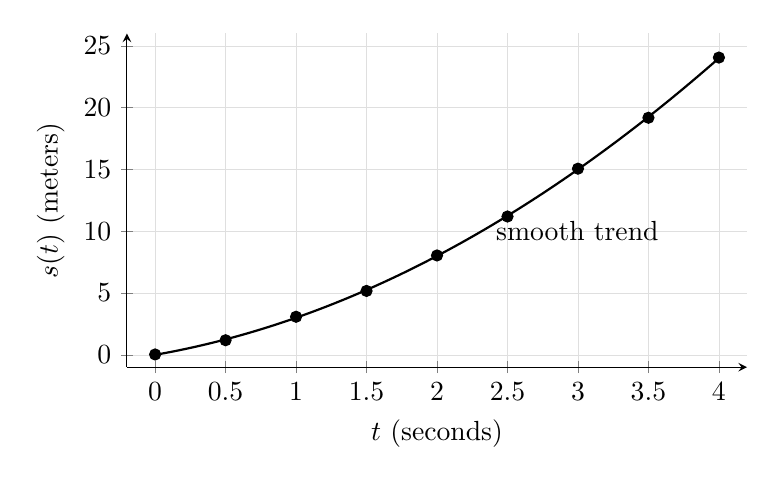
\begin{tikzpicture}
\begin{axis}[
    width=0.78\textwidth,
    height=0.48\textwidth,
    xmin=-0.2, xmax=4.2,
    ymin=-1, ymax=26,
    axis lines=left,
    xlabel={\(t\) (seconds)},
    ylabel={\(s(t)\) (meters)},
    xtick={0,0.5,1,1.5,2,2.5,3,3.5,4},
    ytick={0,5,10,15,20,25},
    grid=both,
    grid style={line width=.1pt, draw=gray!25},
]
\addplot[only marks, mark=*] coordinates {
    (0,0.03)
    (0.5,1.18)
    (1,3.08)
    (1.5,5.17)
    (2,8.04)
    (2.5,11.19)
    (3,15.06)
    (3.5,19.18)
    (4,24.05)
};
\addplot[thick, domain=0:4, samples=80] {x^2+2*x};
\node[anchor=west] at (axis cs:2.35,10) {smooth trend};
\end{axis}
\end{tikzpicture}
\caption{Noisy position data still suggest a smooth motion, but slopes estimated from nearby points can vary.}
\label{fig:noisy-position-data}
\end{figure}

The goal is to estimate the velocity at \(t=2\).

\paragraph{Step 1: one-sided estimates.}
Use the forward difference

\[
\frac{s(2.5)-s(2)}{0.5}
\]

and the backward difference

\[
\frac{s(2)-s(1.5)}{0.5}.
\]

Compute both estimates.  Are they equal?  Should they be?

\paragraph{Step 2: a centered estimate.}
Use the centered difference

\[
\frac{s(2.5)-s(1.5)}{1.0}.
\]

This uses points on both sides of \(t=2\).  Compare it with the two one-sided estimates.

\paragraph{Step 3: a wider centered estimate.}
Use

\[
\frac{s(3.0)-s(1.0)}{2.0}.
\]

This uses data farther away from \(t=2\).  Compare this estimate with the centered estimate from Step 2.

\paragraph{Step 4: repeat at other times.}
Estimate the velocity at \(t=1\) and \(t=3\) using centered differences.

For \(t=1\), use

\[
\frac{s(1.5)-s(0.5)}{1.0}.
\]

For \(t=3\), use

\[
\frac{s(3.5)-s(2.5)}{1.0}.
\]

\paragraph{Step 5: compare with a smooth model.}
The data were produced from a smooth motion close to

\[
s_{\text{true}}(t)=t^2+2t,
\]

with small measurement errors added.

For the smooth model,

\[
v_{\text{true}}(t)=s_{\text{true}}'(t)=2t+2.
\]

Compute

\[
v_{\text{true}}(1),\qquad v_{\text{true}}(2),\qquad v_{\text{true}}(3).
\]

Compare these true velocities with your estimates from the noisy data.

\paragraph{Step 6: the main question.}
A smaller time interval usually gives a better derivative estimate when the data are exact.  But if the measurements are noisy, a very small interval can make the noise more visible because we divide by a small number.

Explain this tension in your own words:

\[
\text{small interval captures local behavior,}
\]

but

\[
\text{small interval can amplify measurement error.}
\]

\paragraph{Optional computing extension.}
Use a graphing tool or spreadsheet.

\begin{enumerate}
\item Plot the data points.

\item Plot the smooth curve

\[
s(t)=t^2+2t
\]

on the same axes.

\item Compute forward, backward, and centered difference estimates at every time where the required neighboring data are available.

\item Make a second plot showing the estimated velocities.

\item Compare the velocity estimates with the line

\[
v(t)=2t+2.
\]
\end{enumerate}

This project is a small version of a real problem.  Scientists often measure position and want velocity.  But measured data are not exact, so the derivative must be estimated with care.

\subsection{Hook: why the definition is not enough}
\label{subsec:hook-definition-not-enough}

The derivative definition is the source of everything in this chapter:

\[
f'(x)=\lim_{h\to0}\frac{f(x+h)-f(x)}{h}.
\]

It tells us what the derivative means.  It proves the first formulas.  It catches corners, cusps, and jumps.  It explains velocity, tangent slope, and local linear approximation.

But it is too slow to use from scratch every time.

For example, consider

\[
F(x)=(x^2+1)(x^3-5).
\]

With the tools of this chapter, we could expand first:

\[
F(x)=x^5+x^3-5x^2-5.
\]

Then we can differentiate term by term:

\[
F'(x)=5x^4+3x^2-10x.
\]

That works here because the product is a polynomial.  But expansion is not always possible or pleasant.  What about

\[
x^2\sqrt{x+1},
\]

or

\[
\frac{x^3+1}{x^2-4},
\]

or, later,

\[
\sin(x^2)?
\]

These functions are built from simpler pieces by multiplying, dividing, and composing.  Their derivatives should be built from the derivatives of those pieces.

The next chapter turns the definition into a working language.  The goal is not to replace meaning with rules.  The goal is to make the meaning fast enough to use.
